\section{Quantifying the Benefits in Crime Reduction} \label{appendix:crime}

\subsection{Data Description}
\label{appendix:crime-data-description}

\noindent The crime data available in ABC/CARE come from four different sources provided by the program, which we supplement with auxiliary datasets. We summarize the ABC/CARE datasets and auxiliary datasets related to crime below. \\

\subsubsection{ABC/CARE Datasets}
\begin{enumerate}
\item Administrative Youth Arrests Dataset.  This dataset is only available for ABC. This dataset records all arrests up to the age at which the data were obtained (April, 1996), when ABC subjects were about 21 years old. The categories of crimes in this dataset are coarser than the ones that we use in the other datasets: it categorizes crimes into property, violent, drug, and miscellaneous crimes. We assume some equivalences, as shown in Table~\ref{tab:crime_cat}.
\item Administrative Adult Arrests Dataset. Gathered when ABC and CARE subjects were around 34 years old, this dataset includes individual data on arrests, with short descriptions of the associated offenses. This dataset includes some subjects for whom the arrest history is missing. To resolve this, we use a methodology (detailed below) involving the sentences data, which does not have missing values.
\item Administrative Sentences Dataset. Gathered when ABC and CARE subjects were about 34 years old, this dataset includes individual data on sentences, with descriptions of the crimes. It also includes total sentence length (projected and actual) and punishment type (jail, prison, parole).
\item Self-reported Adult Crimes Dataset. A module on crimes was included at the age-21 and age-30 interviews for both ABC and CARE. After matching all datasets, we use the information from the self-reported crimes whenever a particular crime does not appear in the other datasets.
\end{enumerate}

\subsubsection{Auxiliary Datasets}
\begin{enumerate}
\item National Crime Victimization Survey (NCVS). The NCVS is a survey (self-reported) on crime victimization reported on the household level. The NCVS does not cover crimes to businesses, and it might under-report crimes that might not be known to all members of a family, such as rape. It also does not give statistics for murders. The data are available from 1993 to 2013. We use NCVS to estimate the total number of victims per type of crime in the U.S., which is used to construct victim-arrest ratios.
\item Uniform Crime Reporting Statistics (UCRS). This dataset contains all crimes that are reported to the police. It contains crimes to households, individuals, and businesses that are captured by most of the law enforcement agencies in the country. We used data from UCRS spanning the years 1996 to 2012. We use UCRS as a complement to NCVS when we estimate the total number of victims per type of crime in the U.S. %We use UCR to construct national arrest-to-sentences and victims-to-arrests ratios for our crime categories.
%\item Bureau of Justice Statistics (BJS): the BJS' Arrest Data Analysis Tool has data on arrests per year per type of crime. This data only includes arrests made by state authorities. There are 133 federal authorities with the jurisdiction to arrest individuals, such as the FBI and Custom and Border Patrol, but this data is not publicly available. As with arrests, there is a distinction between Federal and State sentences given to offenders, depending on whether they were convicted in a state or federal court. We also used the BJS's Offender Sentences tool to acquire data on Federal sentences from 1998 to 2012. It is, however, in more general categories and only includes Violent, Property, Public Order, Drug and Other Offenses.
\item National Judicial Reporting Program (NJRP). We use the NJRP to get data for total number of sentences in the U.S. The data were taken from reports published biennially from 1986 to 2006. We use this dataset to construct arrest-sentence ratios for our crime categories.
\item North Carolina Department of Public Safety dataset (NCDPS). This dataset contains information since 1972 on each individual who is convicted of a crime and enters the state prison system or community supervision in North Carolina. The data do not include arrests, or sentences involving jail or unsupervised probation. Because the North Carolina Department of Public Safety was created 3 years ago to consolidate the state's Department of Correction, Department of Juvenile Justice, and Crime Control, among other state agencies, these data were mostly constructed by the other agencies. We use this dataset to fit a forecasting model that we use to forecast future crimes for ABC/CARE subjects.
\end{enumerate}

\subsubsection{Crime Categories}
\noindent The administrative adult datasets have descriptions of all crimes committed by ABC/CARE subjects. We categorize these crimes to be as comparable as possible to the categories in the other data sources and in the literature on calculating the cost of crime. However, it is inevitable to have some crimes that do not clearly fit into the broad categories. As shown in Table \ref{tab:crime_cat}, the different experimental and auxiliary datasets and the literature use different crime categories. The categorization we present is our effort to make all sources comparable. \\

\begin{table}[H]
\begin{threeparttable}
\scriptsize \caption{Crime Categories} \label{tab:crime_cat}
\begin{tabular}{lllll}
\toprule
{Categories}	&	{Youth Data} & {Costs of Crime} & {Nat. Arrests Data} & {Nat. Sentences Data}	\\
\midrule
%				&				& \cite{mccollister2010cost} 	&			&					\\ \hline
{Arson}			&			& Arson					&	Arson			&					\\	
{Assault}			&	Violent			& Assault				&	Total assaults	& Aggravated 		\\		
				&				&						&					& assaults 			\\ 		
{Burglary}		&				& Household burglary	&	Burglary		& Burglary			\\		
{Fraud}			&				& Fraud					&	Fraud,			& Fraud,			\\		
				&				&						&	Forgery,		& Forgery			\\
				&				&						&	Embezzlement	&					\\		
{Larceny}			&	Property	& Larceny/theft			&	Larceny			& Larceny/theft		\\		
{Miscellaneous}	& 	Drug, Misc.	& 					&	Drug abuse		& Drug offenses		\\		
				&				&						&	total			&					\\ 		
{Vehicle Theft}	&				& MV theft	&	MV theft		& MV theft			\\		
{Murder}			&				& Murder				&	Murder,			& Murder,			\\	
				&				&						& 	Non-negligent 	& Manslaughter		\\
				&				&						& 	manslaughter	&   				\\
{Rape}			&				& Rape/sexual assault	&	Forcible rape, 	& Rape 				\\
				&				&						&	Sex offense		&					\\
{Robbery}			&				& Robbery 				&	Robbery			&					\\
{Vandalism}		&				& Vandalism				&	Vandalism		& 				\\	\bottomrule
\end{tabular}
\begin{tablenotes}
\item Note: This table shows the various measures we have for our categories of crimes from each dataset. ``Costs of Crime'' are from \cite{McCollister_etal_2010_DAD}.
\end{tablenotes}
\end{threeparttable}
\end{table}

\subsection{Methodology for Estimating Crime Costs}
\noindent In this section we give a detailed explanation of the steps taken to calculate the total treatment effect on crime and the costs associated with that effect. We first give a more abstract and formal summary of the process, and then discuss the details for each step. \\
%We follow four steps towards constructing our estimates: (i) First, we count the total number of arrests and sentences for each ABC study individual up to age 34; (ii) then we predict, based on the age 34 count of sentences, the number of sentences that the ABC  individuals will have in the future; (iii) next, based on the two previous points, and on the national victims-to-arrests and arrests-to-sentences ratios for the different categories of crimes we use, we estimate the number of victims that might have suffered (observed and unobserved) crimes by ABC study participants; (iv) finally, using the estimated numbers of victims, we impute costs of the crimes based on the literature. We discuss in detail the different costs associated with criminal activity, and the two main approaches to these calculations as categorized by Bottom-Up and Top-Down methodologies. We now give a more formal summary of those four steps. The details are discussed in the rest of this section.

\begin{enumerate}
\item \textit{Count Arrests and Sentences}. We count the total number of sentences for each subject, $i$, and category of crime (robbery, larceny, etc.), $j$, up to age 34,  which we denote by $S_{i,j}^{34}$. We also match the data on adult arrests, juvenile arrests, and self-reported crimes, to construct total number of  arrests for each crime type up to that age, $A_{i,j}^{34}$. For some subjects, the arrest data are missing. In those cases, we impute the missing data by assuming that the national arrest-sentence ratio for crime type, $j$, is valid for each subject. Let $\overline{A_j}$ be the national total number of arrests for crime type, $j$, and let $\overline{S_j}$ be the national total number of sentences. Then, we construct $r_j=\frac{\overline{A_j}}{\overline{S_j}}$, and we impute $A_{i,j}^{34}=r_j S_{i,j}^{34}$.

\item \textit{Construct Forecasts}. From our external data, we have a dataset to forecast lifetime sentences. In that dataset, we use sentences up to age 34 in all types of crime to forecast future sentences for that crime type, $\widehat{S_{i,j}^{35-50}}$. This gives an estimate of the lifetime sentences as $\widehat{S_{i,j}}=S_{i,j}^{34}+\widehat{S_{i,j}^{35-50}}$. Given that we do not have an analogous dataset to forecast lifetime arrests, we impute the forecasted arrests as a linear function of the forecasted number of sentences: $\widehat{A_{i,j}^{35-50}}=r_j \widehat{S_{i,j}^{35-50}}$. Then, we calculate $\widehat{A_{i,j}}=A_{i,j}^{34}+\widehat{A_{i,j}^{35-50}}$.

\item \textit{Estimate Number of Victims}. Let the national number of victims of a given type of crime be $\overline{V_j}$. We construct a victimization inflation factor for each crime type: $f_j=\frac{\overline{V_j}}{\overline{A_j}}$. It represents the number of times someone is arrested as a fraction of the number of victims of the crimes. Then, the estimated number of victims of subject, $i$, for crime type, $j$, based on arrests is estimated as $\widehat{V_{i,j}^{A}}=A_{i,j}f_j$. For sentences, we calculate an analogous estimate of victims based on the victimization inflation factor and the arrest-sentence ratio: $\widehat{V_{i,j}^{S}}=S_{i,j}f_j r_j$. Both estimates are similar, as we show below. We construct our final estimate of the lifetime victims of subject, $i$, for crime type, $j$, as the average of both estimates to achieve greater precision: $\widehat{V_{i,j}}=\left(\widehat{V_{i,j}^A}+\widehat{V_{i,j}^S}\right)/2$.

\item \textit{Find Total Costs of Crimes}. We use estimates of the cost of crimes for victims from the literature for each crime type $j$, $c_j^V$. We impute the total victim costs of subject, $i$, for crime type, $j$, as $\widehat{C_{i,j}^V}=\widehat{V_{i,j}} c_j^V$. We also calculate different costs from the justice system (including police) associated with the different crime types, but only for the ones that included arrests or sentences (i.e. we do not consider the victimization inflation), as: $C_{i,j}^{JS}=\widehat{A_{i,j}} c_j^{JS}$. Finally, we also construct the total costs of incarceration for crime type, $j$, $\widehat{C_{i,j}^{P}}$ as the total time the subject was imprisoned for that type of crime, $P_{i,j}$, multiplied by the cost of a day in prison $c_P$. All of our cost estimates are discounted to birth.
\end{enumerate}


\subsubsection{Count Arrests and Sentences}
\noindent Unlike previous studies, we use several datasets to construct measures of criminal activity of the ABC/CARE subject. We generate a count of the number of arrests and of the number of sentences by crime category for each ABC/CARE subject. We start by counting sentences, which is trivial, as we have complete information on sentences for all ABC/CARE subjects in one dataset. \\

\noindent Unlike counting sentences, the count of arrests is more involved.\footnote{Throughout this appendix, for all the calculations involving counting arrests, if the arrest was the result of more than one \textit{offense}, we count the number and type of offenses separately, rather than counting all of them as one. An offense is the precise definition for the unit that we work with.} We now describe the procedure we follow to get a count of arrests that is as complete as possible. We begin by matching, based on crime description and date, the arrests from the adult administrative data, the youth administrative data, and the self-reported dataset. It is possible that the adult data are missing youth arrests that were expunged from the criminal records or crimes committed in states other than North Carolina, which were not obtained in the collection of administrative data. Because we observe the arrest dates, we confirm that we are not duplicating any arrests. To align the youth arrests data, which are categorized more broadly, we assume that all violent crimes are assaults (the most common category of violent crime in the sample) and that all property crimes are larcenies (the most common category of property crime). We categorize both drug and miscellaneous crimes in the miscellaneous category, for which we do not compute victim costs. \\
%The original number of arrests in the data was 444. Both the youth administrative data and the self-reported arrests were matched in a case-by case basis with the administrative arrest records, thus making the pre-1995 records much more complete. The number of arrests in the data after the matching and elimination of overlapping arrests is 794.

\noindent The main problem we confront with these data is that there are some individuals who are missing data on arrests in the data collected at age 34. We know this is the case because there are sentences for which we do not observe the corresponding arrests. While this is expected for some crimes, such as speeding or shoplifting, it is not possible for others. This seems to be due to the difficulty in collecting administrative information on arrests. Counting arrests using many data sources eases  reconstruction of adult arrests data. We tackle this challenge by first identifying those individuals who should have arrests, because they have sentences that necessarily imply they were arrested at some point of time. Then we impute the number of arrests for each of those sentences, based on the national arrest-sentence ratio. We estimate that 11 individuals (10\% of the ABC sample) have missing arrest data. We note that the final estimates of effects on reduction in crime costs using only sentences (which do not have any missing values) are very similar to the ones using arrests. \\

\noindent The effect of adding the different datasets, as well as the final counts of both arrests and sentences is presented in Figure \ref{fig:datagraph}. The first three pairs of bars present the number of additional crimes included in the data by the addition of the self-reported, juvenile, and sentences datasets. In the case of sentences, we first show the effect of imputing just one arrest per sentence, and only for individuals with missing arrests. Notice that the juvenile data only adds assaults, larcenies, and miscellaneous, as discussed above. The next pair of bars shows the effect of adding more than one arrest per sentence for the individuals with missing data, using the arrest-sentence ratios. The effect is significant, adding about 30\% more crimes to the previous estimate. Importantly, some rape arrests are added to the control group in this step, because of one subject who presented a sentence for that crime. Finally, the total number of sentences is far lower than the total number of arrests, even if only the original arrests are counted. We also note in this chart that the volume of the crimes is mostly driven by miscellaneous crimes (which are mostly drug and traffic crimes). As these crimes are counted as victimless in our methodology, their effect on the final estimates is much smaller than what this chart might suggest. \\

\begin{figure}[H]
\caption{Counts of Arrests and Sentences}
\centering \label{fig:datagraph}
{\scalebox{0.8}{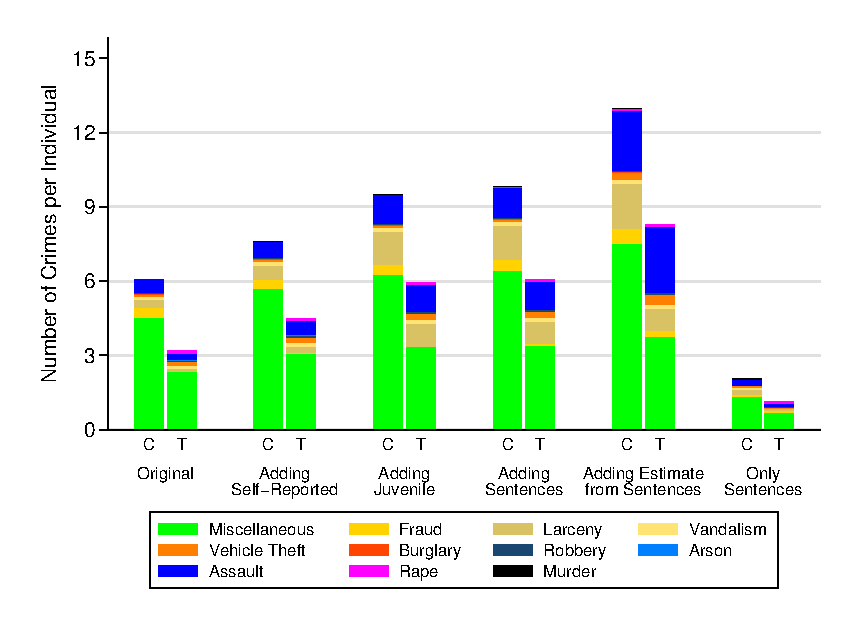
\includegraphics{AppOutput/Crime/counts_misc}}}
\floatfoot{
\footnotesize
\noindent Note: This chart shows the arrests per capita for the control (C) and treatment (T) groups. The first pair of bars shows the original arrests data from the administrative adult dataset. The next pair adds the self-reported crimes that did not match with the original arrests data. The next pair adds data from the administrative juvenile dataset that did not match with the previous datasets. The next pair adds one arrest for every sentence that did not match with the previous datasets and one arrest for every sentence that had arrest data missing. The next pair adds $n$ arrests instead of one for each sentence, where $n$ is calculated using the arrest-sentence ratio obtained from auxiliary datasets. The final pair of bars, for reference, is the total number of sentences from the administrative sentences dataset.
}
\end{figure}

\subsubsection{Construct Forecasts}

\noindent The data available describe the ABC/CARE subjects' crimes committed up to age 34. However, we believe that the effect of the programs on crime does not stop at that age. To forecast the number of crimes that the study participants commit beyond age 34, we use data from the North Carolina Department of Public Safety (NCDPS). Because the crime data are obtained from the same state in which ABC/CARE were implemented, the forecasting model is appropriate for the ABC/CARE samples. To the best of our knowledge, no study of the effects of an early childhood education program has ever used microdata to estimate a predictive model for future crimes. The estimations in \cite{Heckman_Moon_etal_2010_RateofReturn} are based on national age ratios (crimes of a certain category committed by older people over crimes of the same category committed by younger people at a specific time), rather than on microdata. However, age ratios only consider the same category of crime as an input to the estimation model and the results can reflect demographic transitions.

It would be ideal to use forecasting models estimated from the same cohorts as the ABC/CARE subjects. However, it is not possible to forecast crimes committed until older ages because the ABC/CARE subjects are currently about 46 years old. To forecast crimes at older ages, it is necessary to use earlier cohorts. The data are available from 1972 (44 years ago as of 2016), and thus they do not contain a complete criminal history for any cohort of individuals.
%Given that, we have to choose specific cohorts for the estimations, such that they are old enough to cover the ages we need to predict, and young enough to have their entire crime life covered in the dataset, in the same way as the entire crime life of ABC individuals in covered in our data. In particular,
We assume that few crimes are committed after the age of 50. \\
%, and that crime life does not start until age 16.
 We separately estimate predictions from ages 35-40, 40-45, and 45-50. We have plentiful observations to estimate crimes in all the age ranges. %\footnote{As an example, to predict crimes at ages 45-50 we need individuals aged 50+. To have enough birth year cohorts, we consider individuals aged 50-59 in 2015. The oldest of these individuals were aged 16 in 1972, so we can reasonably expect them to having committed few crimes before that year. Finding observations for crime predictions at earlier ages is even easier.}
%Age 5 in 2015-->Age 12 in 1972.            Age 50 in 2015-->Age 16 in 1972.
%Age 55 in 2015-->Age 12 in 1972.            Age 59 in 2015-->Age 16 in 1972.
We calculate our forecasts using a five-step procedure:
\begin{enumerate}
\item Find individuals that are at least 40 years old as of 2016 in the NCDPS dataset.
\item Regress the number of crimes of each type at ages 35--40 on those at ages 16--34.
\item Use the estimated forecasting model for ABC individuals, attributing those crimes to age 40 for discounting purposes.
\item Repeat the three previous steps for ages 40--45 and 45--50. %50-55?
\item For individuals with no criminal histories before age 34, assume that they commit no crimes after 34.
\end{enumerate}

%include more tables if ages 55 are covered, not just 50
\begin{sidewaystable}[H]
\caption{NCDPS Regressions of Ages 35--40 on Ages 16--35, Females} \label{tab:reg1f}
\begin{adjustbox}{max width=\textwidth}
\begin{threeparttable}
\begin{tabular}{lccccccccccc}
\hline\hline \noalign{\smallskip} & Miscellaneous & Fraud & Larceny & Vandalism & Auto Theft & Burglary & Robbery & Arson & Assault & Rape & Murder\\
\noalign{\smallskip}\hline \noalign{\smallskip}Miscellaneous & 0.103 & -0.029 & 0.009 & 0.001 & 0.001 & 0.001 & 0.000 & -0.000 & 0.002 & -0.000 & -0.001\\
 & \begin{footnotesize}(27.71)**\end{footnotesize} & \begin{footnotesize}(5.90)**\end{footnotesize} & \begin{footnotesize}(6.00)**\end{footnotesize} & \begin{footnotesize}(3.88)**\end{footnotesize} & \begin{footnotesize}(5.18)**\end{footnotesize} & \begin{footnotesize}(2.25)*\end{footnotesize} & \begin{footnotesize}(1.91)\end{footnotesize} & \begin{footnotesize}(0.62)\end{footnotesize} & \begin{footnotesize}(3.16)**\end{footnotesize} & \begin{footnotesize}(1.27)\end{footnotesize} & \begin{footnotesize}(2.85)**\end{footnotesize}\\
\noalign{\smallskip}Fraud & -0.047 & 0.104 & 0.003 & -0.000 & 0.000 & 0.000 & 0.000 & 0.000 & -0.001 & -0.000 & -0.000\\
 & \begin{footnotesize}(21.71)**\end{footnotesize} & \begin{footnotesize}(36.61)**\end{footnotesize} & \begin{footnotesize}(3.81)**\end{footnotesize} & \begin{footnotesize}(2.31)*\end{footnotesize} & \begin{footnotesize}(0.60)\end{footnotesize} & \begin{footnotesize}(2.02)*\end{footnotesize} & \begin{footnotesize}(0.02)\end{footnotesize} & \begin{footnotesize}(1.76)\end{footnotesize} & \begin{footnotesize}(1.48)\end{footnotesize} & \begin{footnotesize}(0.75)\end{footnotesize} & \begin{footnotesize}(1.72)\end{footnotesize}\\
\noalign{\smallskip}Larceny & 0.034 & 0.002 & 0.105 & 0.001 & 0.002 & 0.002 & 0.001 & 0.000 & 0.004 & 0.000 & -0.000\\
 & \begin{footnotesize}(8.16)**\end{footnotesize} & \begin{footnotesize}(0.33)\end{footnotesize} & \begin{footnotesize}(62.36)**\end{footnotesize} & \begin{footnotesize}(2.37)*\end{footnotesize} & \begin{footnotesize}(10.35)**\end{footnotesize} & \begin{footnotesize}(7.80)**\end{footnotesize} & \begin{footnotesize}(5.97)**\end{footnotesize} & \begin{footnotesize}(2.99)**\end{footnotesize} & \begin{footnotesize}(5.65)**\end{footnotesize} & \begin{footnotesize}(1.30)\end{footnotesize} & \begin{footnotesize}(1.67)\end{footnotesize}\\
\noalign{\smallskip}Vandal & 0.000 & -0.036 & -0.024 & 0.012 & 0.004 & 0.007 & 0.005 & 0.003 & 0.043 & 0.000 & -0.000\\
 & \begin{footnotesize}(0.01)\end{footnotesize} & \begin{footnotesize}(1.10)\end{footnotesize} & \begin{footnotesize}(2.43)*\end{footnotesize} & \begin{footnotesize}(6.40)**\end{footnotesize} & \begin{footnotesize}(2.86)**\end{footnotesize} & \begin{footnotesize}(3.87)**\end{footnotesize} & \begin{footnotesize}(3.34)**\end{footnotesize} & \begin{footnotesize}(3.40)**\end{footnotesize} & \begin{footnotesize}(9.27)**\end{footnotesize} & \begin{footnotesize}(0.79)\end{footnotesize} & \begin{footnotesize}(0.23)\end{footnotesize}\\
\noalign{\smallskip}Auto Theft & 0.059 & -0.026 & 0.055 & 0.004 & 0.012 & 0.007 & 0.005 & -0.002 & -0.014 & -0.000 & 0.002\\
 & \begin{footnotesize}(1.55)\end{footnotesize} & \begin{footnotesize}(0.52)\end{footnotesize} & \begin{footnotesize}(3.57)**\end{footnotesize} & \begin{footnotesize}(1.28)\end{footnotesize} & \begin{footnotesize}(5.94)**\end{footnotesize} & \begin{footnotesize}(2.48)*\end{footnotesize} & \begin{footnotesize}(2.52)*\end{footnotesize} & \begin{footnotesize}(1.30)\end{footnotesize} & \begin{footnotesize}(2.02)*\end{footnotesize} & \begin{footnotesize}(0.23)\end{footnotesize} & \begin{footnotesize}(1.02)\end{footnotesize}\\
\noalign{\smallskip}Burglary & 0.049 & -0.031 & 0.011 & 0.002 & 0.006 & 0.044 & 0.000 & -0.001 & -0.003 & -0.000 & -0.001\\
 & \begin{footnotesize}(1.77)\end{footnotesize} & \begin{footnotesize}(0.86)\end{footnotesize} & \begin{footnotesize}(1.01)\end{footnotesize} & \begin{footnotesize}(0.95)\end{footnotesize} & \begin{footnotesize}(3.86)**\end{footnotesize} & \begin{footnotesize}(22.56)**\end{footnotesize} & \begin{footnotesize}(0.20)\end{footnotesize} & \begin{footnotesize}(1.26)\end{footnotesize} & \begin{footnotesize}(0.55)\end{footnotesize} & \begin{footnotesize}(0.25)\end{footnotesize} & \begin{footnotesize}(0.34)\end{footnotesize}\\
\noalign{\smallskip}Robbery & 0.030 & 0.054 & 0.040 & 0.002 & 0.005 & -0.001 & 0.028 & 0.002 & -0.000 & -0.000 & 0.002\\
 & \begin{footnotesize}(1.05)\end{footnotesize} & \begin{footnotesize}(1.46)\end{footnotesize} & \begin{footnotesize}(3.51)**\end{footnotesize} & \begin{footnotesize}(1.03)\end{footnotesize} & \begin{footnotesize}(3.43)**\end{footnotesize} & \begin{footnotesize}(0.28)\end{footnotesize} & \begin{footnotesize}(17.69)**\end{footnotesize} & \begin{footnotesize}(2.22)*\end{footnotesize} & \begin{footnotesize}(0.07)\end{footnotesize} & \begin{footnotesize}(0.29)\end{footnotesize} & \begin{footnotesize}(1.50)\end{footnotesize}\\
\noalign{\smallskip}Arson & 0.070 & -0.087 & -0.035 & 0.008 & 0.011 & 0.006 & 0.025 & 0.010 & 0.017 & -0.000 & 0.005\\
 & \begin{footnotesize}(1.29)\end{footnotesize} & \begin{footnotesize}(1.22)\end{footnotesize} & \begin{footnotesize}(1.61)\end{footnotesize} & \begin{footnotesize}(1.98)*\end{footnotesize} & \begin{footnotesize}(3.98)**\end{footnotesize} & \begin{footnotesize}(1.62)\end{footnotesize} & \begin{footnotesize}(8.19)**\end{footnotesize} & \begin{footnotesize}(4.95)**\end{footnotesize} & \begin{footnotesize}(1.67)\end{footnotesize} & \begin{footnotesize}(0.19)\end{footnotesize} & \begin{footnotesize}(1.60)\end{footnotesize}\\
\noalign{\smallskip}Assault & 0.064 & -0.060 & 0.007 & 0.007 & 0.001 & 0.002 & -0.000 & 0.002 & 0.048 & -0.000 & 0.000\\
 & \begin{footnotesize}(5.74)**\end{footnotesize} & \begin{footnotesize}(4.11)**\end{footnotesize} & \begin{footnotesize}(1.63)\end{footnotesize} & \begin{footnotesize}(7.82)**\end{footnotesize} & \begin{footnotesize}(1.83)\end{footnotesize} & \begin{footnotesize}(1.93)\end{footnotesize} & \begin{footnotesize}(0.14)\end{footnotesize} & \begin{footnotesize}(4.52)**\end{footnotesize} & \begin{footnotesize}(22.78)**\end{footnotesize} & \begin{footnotesize}(0.36)\end{footnotesize} & \begin{footnotesize}(0.34)\end{footnotesize}\\
\noalign{\smallskip}Rape & -0.015 & -0.131 & -0.003 & -0.003 & -0.003 & -0.004 & -0.006 & -0.001 & 0.001 & -0.000 & -0.002\\
 & \begin{footnotesize}(0.15)\end{footnotesize} & \begin{footnotesize}(0.98)\end{footnotesize} & \begin{footnotesize}(0.08)\end{footnotesize} & \begin{footnotesize}(0.42)\end{footnotesize} & \begin{footnotesize}(0.49)\end{footnotesize} & \begin{footnotesize}(0.55)\end{footnotesize} & \begin{footnotesize}(0.99)\end{footnotesize} & \begin{footnotesize}(0.24)\end{footnotesize} & \begin{footnotesize}(0.08)\end{footnotesize} & \begin{footnotesize}(0.06)\end{footnotesize} & \begin{footnotesize}(0.33)\end{footnotesize}\\
\noalign{\smallskip}Murder & 0.006 & -0.166 & -0.008 & 0.003 & -0.002 & -0.002 & -0.002 & 0.003 & 0.001 & -0.000 & -0.001\\
 & \begin{footnotesize}(0.16)\end{footnotesize} & \begin{footnotesize}(3.44)**\end{footnotesize} & \begin{footnotesize}(0.54)\end{footnotesize} & \begin{footnotesize}(1.19)\end{footnotesize} & \begin{footnotesize}(0.94)\end{footnotesize} & \begin{footnotesize}(0.75)\end{footnotesize} & \begin{footnotesize}(1.22)\end{footnotesize} & \begin{footnotesize}(2.24)*\end{footnotesize} & \begin{footnotesize}(0.12)\end{footnotesize} & \begin{footnotesize}(0.34)\end{footnotesize} & \begin{footnotesize}(0.37)\end{footnotesize}\\
\noalign{\smallskip}constant & 0.069 & 0.267 & 0.041 & 0.004 & 0.001 & 0.001 & 0.001 & 0.001 & 0.023 & 0.000 & 0.004\\
 & \begin{footnotesize}(13.39)**\end{footnotesize} & \begin{footnotesize}(39.01)**\end{footnotesize} & \begin{footnotesize}(19.54)**\end{footnotesize} & \begin{footnotesize}(10.27)**\end{footnotesize} & \begin{footnotesize}(2.76)**\end{footnotesize} & \begin{footnotesize}(3.17)**\end{footnotesize} & \begin{footnotesize}(4.80)**\end{footnotesize} & \begin{footnotesize}(3.52)**\end{footnotesize} & \begin{footnotesize}(23.81)**\end{footnotesize} & \begin{footnotesize}(3.38)**\end{footnotesize} & \begin{footnotesize}(12.90)**\end{footnotesize}\\
\noalign{\smallskip}$R^2$ & 0.02 & 0.02 & 0.07 & 0.00 & 0.01 & 0.01 & 0.01 & 0.00 & 0.01 & 0.00 & 0.00\\
$N$ & 63,515 & 63,515 & 63,515 & 63,515 & 63,515 & 63,515 & 63,515 & 63,515 & 63,515 & 63,515 & 63,515\\
\noalign{\smallskip}\hline\hline\end{tabular}

\begin{tablenotes}
\item Note: This table shows how the crimes at ages 35--40 (in the columns) are predicted by crimes at ages 16--35 (in the rows). The estimations are predicted using the North Carolina Department of Public Safety dataset, which contains information on all individuals that have ever been sentenced in North Carolina. We use linear regressions in all cases. The sample for this model is limited to individuals who are at least 40 years old. *~$p<0.05$; **~$p<0.01$.
\end{tablenotes}
\end{threeparttable}
\end{adjustbox}
\end{sidewaystable}


\begin{sidewaystable}[H]
\caption{NCDPS Regressions of Ages 35--40 on Ages 16--35, Males} \label{tab:reg1m}
\begin{adjustbox}{max width=\textwidth}
\begin{threeparttable}
\begin{tabular}{lccccccccccc}
\hline\hline \noalign{\smallskip} & Miscellaneous & Fraud & Larceny & Vandalism & Auto Theft & Burglary & Robbery & Arson & Assault & Rape & Murder\\
\noalign{\smallskip}\hline \noalign{\smallskip}Miscellaneous & 0.095 & -0.002 & 0.004 & 0.000 & 0.001 & 0.001 & 0.000 & -0.000 & 0.005 & -0.001 & -0.001\\
 & \begin{footnotesize}(73.29)**\end{footnotesize} & \begin{footnotesize}(2.13)*\end{footnotesize} & \begin{footnotesize}(8.97)**\end{footnotesize} & \begin{footnotesize}(2.71)**\end{footnotesize} & \begin{footnotesize}(6.47)**\end{footnotesize} & \begin{footnotesize}(5.87)**\end{footnotesize} & \begin{footnotesize}(1.50)\end{footnotesize} & \begin{footnotesize}(0.12)\end{footnotesize} & \begin{footnotesize}(14.73)**\end{footnotesize} & \begin{footnotesize}(3.28)**\end{footnotesize} & \begin{footnotesize}(5.83)**\end{footnotesize}\\
\noalign{\smallskip}Fraud & -0.025 & 0.107 & 0.007 & 0.000 & 0.001 & 0.002 & 0.001 & -0.000 & -0.000 & -0.000 & -0.000\\
 & \begin{footnotesize}(13.76)**\end{footnotesize} & \begin{footnotesize}(67.23)**\end{footnotesize} & \begin{footnotesize}(11.68)**\end{footnotesize} & \begin{footnotesize}(0.47)\end{footnotesize} & \begin{footnotesize}(3.44)**\end{footnotesize} & \begin{footnotesize}(5.27)**\end{footnotesize} & \begin{footnotesize}(2.53)*\end{footnotesize} & \begin{footnotesize}(0.61)\end{footnotesize} & \begin{footnotesize}(0.34)\end{footnotesize} & \begin{footnotesize}(0.35)\end{footnotesize} & \begin{footnotesize}(1.96)*\end{footnotesize}\\
\noalign{\smallskip}Larceny & 0.041 & 0.012 & 0.092 & 0.001 & 0.005 & 0.010 & 0.004 & 0.000 & 0.009 & -0.000 & -0.000\\
 & \begin{footnotesize}(14.34)**\end{footnotesize} & \begin{footnotesize}(4.83)**\end{footnotesize} & \begin{footnotesize}(97.06)**\end{footnotesize} & \begin{footnotesize}(5.13)**\end{footnotesize} & \begin{footnotesize}(14.85)**\end{footnotesize} & \begin{footnotesize}(19.72)**\end{footnotesize} & \begin{footnotesize}(12.30)**\end{footnotesize} & \begin{footnotesize}(1.79)\end{footnotesize} & \begin{footnotesize}(11.37)**\end{footnotesize} & \begin{footnotesize}(0.46)\end{footnotesize} & \begin{footnotesize}(0.59)\end{footnotesize}\\
\noalign{\smallskip}Vandal & 0.041 & -0.017 & -0.007 & 0.019 & 0.002 & 0.002 & 0.002 & 0.002 & 0.029 & 0.001 & 0.000\\
 & \begin{footnotesize}(4.51)**\end{footnotesize} & \begin{footnotesize}(2.13)*\end{footnotesize} & \begin{footnotesize}(2.22)*\end{footnotesize} & \begin{footnotesize}(23.49)**\end{footnotesize} & \begin{footnotesize}(1.96)\end{footnotesize} & \begin{footnotesize}(1.06)\end{footnotesize} & \begin{footnotesize}(1.76)\end{footnotesize} & \begin{footnotesize}(5.41)**\end{footnotesize} & \begin{footnotesize}(11.26)**\end{footnotesize} & \begin{footnotesize}(1.06)\end{footnotesize} & \begin{footnotesize}(0.62)\end{footnotesize}\\
\noalign{\smallskip}Auto Theft & 0.015 & 0.014 & 0.005 & 0.002 & 0.043 & 0.013 & 0.000 & 0.000 & 0.008 & 0.001 & 0.001\\
 & \begin{footnotesize}(1.58)\end{footnotesize} & \begin{footnotesize}(1.70)\end{footnotesize} & \begin{footnotesize}(1.48)\end{footnotesize} & \begin{footnotesize}(1.86)\end{footnotesize} & \begin{footnotesize}(39.51)**\end{footnotesize} & \begin{footnotesize}(7.87)**\end{footnotesize} & \begin{footnotesize}(0.14)\end{footnotesize} & \begin{footnotesize}(0.13)\end{footnotesize} & \begin{footnotesize}(3.12)**\end{footnotesize} & \begin{footnotesize}(1.28)\end{footnotesize} & \begin{footnotesize}(1.18)\end{footnotesize}\\
\noalign{\smallskip}Burglary & 0.005 & 0.011 & 0.010 & 0.002 & 0.004 & 0.040 & 0.003 & -0.000 & 0.003 & 0.001 & -0.000\\
 & \begin{footnotesize}(1.26)\end{footnotesize} & \begin{footnotesize}(3.06)**\end{footnotesize} & \begin{footnotesize}(6.86)**\end{footnotesize} & \begin{footnotesize}(4.33)**\end{footnotesize} & \begin{footnotesize}(9.17)**\end{footnotesize} & \begin{footnotesize}(52.89)**\end{footnotesize} & \begin{footnotesize}(6.55)**\end{footnotesize} & \begin{footnotesize}(0.30)\end{footnotesize} & \begin{footnotesize}(2.34)*\end{footnotesize} & \begin{footnotesize}(2.37)*\end{footnotesize} & \begin{footnotesize}(0.73)\end{footnotesize}\\
\noalign{\smallskip}Robbery & -0.032 & 0.000 & 0.011 & 0.000 & 0.003 & 0.006 & 0.019 & -0.000 & -0.000 & 0.000 & 0.001\\
 & \begin{footnotesize}(5.06)**\end{footnotesize} & \begin{footnotesize}(0.01)\end{footnotesize} & \begin{footnotesize}(5.42)**\end{footnotesize} & \begin{footnotesize}(0.67)\end{footnotesize} & \begin{footnotesize}(4.61)**\end{footnotesize} & \begin{footnotesize}(5.67)**\end{footnotesize} & \begin{footnotesize}(26.50)**\end{footnotesize} & \begin{footnotesize}(1.00)\end{footnotesize} & \begin{footnotesize}(0.21)\end{footnotesize} & \begin{footnotesize}(0.00)\end{footnotesize} & \begin{footnotesize}(1.68)\end{footnotesize}\\
\noalign{\smallskip}Arson & 0.008 & -0.023 & -0.010 & 0.012 & -0.004 & 0.008 & 0.004 & 0.007 & 0.031 & -0.001 & 0.001\\
 & \begin{footnotesize}(0.26)\end{footnotesize} & \begin{footnotesize}(0.82)\end{footnotesize} & \begin{footnotesize}(0.95)\end{footnotesize} & \begin{footnotesize}(4.40)**\end{footnotesize} & \begin{footnotesize}(0.98)\end{footnotesize} & \begin{footnotesize}(1.44)\end{footnotesize} & \begin{footnotesize}(1.22)\end{footnotesize} & \begin{footnotesize}(6.73)**\end{footnotesize} & \begin{footnotesize}(3.49)**\end{footnotesize} & \begin{footnotesize}(0.21)\end{footnotesize} & \begin{footnotesize}(0.39)\end{footnotesize}\\
\noalign{\smallskip}Assault & 0.041 & -0.010 & -0.000 & 0.005 & -0.001 & 0.000 & 0.002 & 0.000 & 0.051 & 0.001 & 0.001\\
 & \begin{footnotesize}(11.14)**\end{footnotesize} & \begin{footnotesize}(3.18)**\end{footnotesize} & \begin{footnotesize}(0.09)\end{footnotesize} & \begin{footnotesize}(15.94)**\end{footnotesize} & \begin{footnotesize}(1.60)\end{footnotesize} & \begin{footnotesize}(0.12)\end{footnotesize} & \begin{footnotesize}(4.47)**\end{footnotesize} & \begin{footnotesize}(2.56)*\end{footnotesize} & \begin{footnotesize}(49.57)**\end{footnotesize} & \begin{footnotesize}(3.43)**\end{footnotesize} & \begin{footnotesize}(3.29)**\end{footnotesize}\\
\noalign{\smallskip}Rape & -0.003 & -0.016 & -0.010 & -0.002 & -0.002 & -0.006 & -0.002 & -0.000 & -0.004 & 0.011 & -0.001\\
 & \begin{footnotesize}(0.33)\end{footnotesize} & \begin{footnotesize}(1.77)\end{footnotesize} & \begin{footnotesize}(2.86)**\end{footnotesize} & \begin{footnotesize}(2.32)*\end{footnotesize} & \begin{footnotesize}(1.72)\end{footnotesize} & \begin{footnotesize}(3.42)**\end{footnotesize} & \begin{footnotesize}(1.66)\end{footnotesize} & \begin{footnotesize}(0.54)\end{footnotesize} & \begin{footnotesize}(1.21)\end{footnotesize} & \begin{footnotesize}(8.61)**\end{footnotesize} & \begin{footnotesize}(1.69)\end{footnotesize}\\
\noalign{\smallskip}Murder & -0.086 & -0.053 & -0.025 & -0.002 & -0.004 & -0.011 & -0.001 & -0.001 & -0.007 & -0.003 & 0.003\\
 & \begin{footnotesize}(6.33)**\end{footnotesize} & \begin{footnotesize}(4.45)**\end{footnotesize} & \begin{footnotesize}(5.51)**\end{footnotesize} & \begin{footnotesize}(1.71)\end{footnotesize} & \begin{footnotesize}(2.54)*\end{footnotesize} & \begin{footnotesize}(4.31)**\end{footnotesize} & \begin{footnotesize}(0.87)\end{footnotesize} & \begin{footnotesize}(1.53)\end{footnotesize} & \begin{footnotesize}(1.79)\end{footnotesize} & \begin{footnotesize}(1.56)\end{footnotesize} & \begin{footnotesize}(3.35)**\end{footnotesize}\\
\noalign{\smallskip}constant & 0.213 & 0.124 & 0.031 & 0.005 & 0.004 & 0.011 & 0.006 & 0.001 & 0.048 & 0.009 & 0.006\\
 & \begin{footnotesize}(69.25)**\end{footnotesize} & \begin{footnotesize}(45.55)**\end{footnotesize} & \begin{footnotesize}(29.74)**\end{footnotesize} & \begin{footnotesize}(18.57)**\end{footnotesize} & \begin{footnotesize}(10.95)**\end{footnotesize} & \begin{footnotesize}(19.97)**\end{footnotesize} & \begin{footnotesize}(17.78)**\end{footnotesize} & \begin{footnotesize}(9.22)**\end{footnotesize} & \begin{footnotesize}(55.54)**\end{footnotesize} & \begin{footnotesize}(24.70)**\end{footnotesize} & \begin{footnotesize}(27.76)**\end{footnotesize}\\
\noalign{\smallskip}$R^2$ & 0.03 & 0.02 & 0.05 & 0.01 & 0.01 & 0.02 & 0.01 & 0.00 & 0.02 & 0.00 & 0.00\\
$N$ & 230,706 & 230,706 & 230,706 & 230,706 & 230,706 & 230,706 & 230,706 & 230,706 & 230,706 & 230,706 & 230,706\\
\noalign{\smallskip}\hline\hline\end{tabular}

\begin{tablenotes}
\item Note: This table shows how the crimes at ages 35--40 (in the columns) are predicted by crimes at ages 16--35 (in the rows). The estimations are predicted using the North Carolina Department of Public Safety dataset, which contains information on all individuals that have ever been sentenced in North Carolina. We use linear regressions in all cases. The sample for this model is limited to individuals who are at least 40 years old. *~$p<0.05$; **~$p<0.01$.
\end{tablenotes}
\end{threeparttable}
\end{adjustbox}
\end{sidewaystable}

\begin{sidewaystable}[H]
\caption{NCDPS Regressions of Ages 40--45 on Ages 16--35, Females} \label{tab:reg2f}
\begin{adjustbox}{max width=\textwidth}
\begin{threeparttable}
\begin{tabular}{lccccccccccc}
\toprule \noalign{\smallskip} & Miscellaneous & Fraud & Larceny & Vandalism & Auto Theft & Burglary & Robbery & Arson & Assault & Rape & Murder\\
\noalign{\smallskip}\midrule \noalign{\smallskip}Miscellaneous & 0.020 & -0.006 & -0.001 & 0.000 & 0.000 & 0.000 & -0.000 & 0.000 & 0.001 & 0.000 & -0.001\\
 & \begin{footnotesize}(4.33)**\end{footnotesize} & \begin{footnotesize}(5.18)**\end{footnotesize} & \begin{footnotesize}(0.85)\end{footnotesize} & \begin{footnotesize}(0.78)\end{footnotesize} & \begin{footnotesize}(0.46)\end{footnotesize} & \begin{footnotesize}(1.29)\end{footnotesize} & \begin{footnotesize}(0.11)\end{footnotesize} & \begin{footnotesize}(0.84)\end{footnotesize} & \begin{footnotesize}(0.64)\end{footnotesize} & \begin{footnotesize}(3.66)**\end{footnotesize} & \begin{footnotesize}(2.65)**\end{footnotesize}\\
\noalign{\smallskip}Fraud & 0.046 & 0.003 & 0.002 & 0.000 & 0.001 & -0.000 & 0.000 & -0.000 & -0.000 & 0.000 & -0.000\\
 & \begin{footnotesize}(19.30)**\end{footnotesize} & \begin{footnotesize}(4.41)**\end{footnotesize} & \begin{footnotesize}(2.86)**\end{footnotesize} & \begin{footnotesize}(1.50)\end{footnotesize} & \begin{footnotesize}(4.86)**\end{footnotesize} & \begin{footnotesize}(0.56)\end{footnotesize} & \begin{footnotesize}(1.62)\end{footnotesize} & \begin{footnotesize}(0.62)\end{footnotesize} & \begin{footnotesize}(1.13)\end{footnotesize} & \begin{footnotesize}(2.50)*\end{footnotesize} & \begin{footnotesize}(0.44)\end{footnotesize}\\
\noalign{\smallskip}Larceny & 0.025 & -0.002 & 0.070 & 0.000 & 0.001 & 0.002 & 0.000 & -0.000 & 0.004 & -0.000 & -0.000\\
 & \begin{footnotesize}(5.12)**\end{footnotesize} & \begin{footnotesize}(1.54)\end{footnotesize} & \begin{footnotesize}(41.35)**\end{footnotesize} & \begin{footnotesize}(0.06)\end{footnotesize} & \begin{footnotesize}(3.61)**\end{footnotesize} & \begin{footnotesize}(6.68)**\end{footnotesize} & \begin{footnotesize}(0.75)\end{footnotesize} & \begin{footnotesize}(1.27)\end{footnotesize} & \begin{footnotesize}(5.02)**\end{footnotesize} & \begin{footnotesize}(0.45)\end{footnotesize} & \begin{footnotesize}(0.45)\end{footnotesize}\\
\noalign{\smallskip}Vandal & -0.016 & -0.009 & -0.018 & 0.002 & -0.001 & 0.005 & 0.001 & 0.003 & 0.019 & -0.000 & -0.001\\
 & \begin{footnotesize}(0.52)\end{footnotesize} & \begin{footnotesize}(1.22)\end{footnotesize} & \begin{footnotesize}(1.71)\end{footnotesize} & \begin{footnotesize}(1.02)\end{footnotesize} & \begin{footnotesize}(0.58)\end{footnotesize} & \begin{footnotesize}(2.66)**\end{footnotesize} & \begin{footnotesize}(0.38)\end{footnotesize} & \begin{footnotesize}(3.06)**\end{footnotesize} & \begin{footnotesize}(3.54)**\end{footnotesize} & \begin{footnotesize}(0.71)\end{footnotesize} & \begin{footnotesize}(0.49)\end{footnotesize}\\
\noalign{\smallskip}Auto Theft & 0.012 & -0.011 & 0.010 & 0.004 & 0.012 & 0.013 & -0.001 & -0.001 & -0.017 & 0.007 & 0.001\\
 & \begin{footnotesize}(0.25)\end{footnotesize} & \begin{footnotesize}(0.87)\end{footnotesize} & \begin{footnotesize}(0.56)\end{footnotesize} & \begin{footnotesize}(0.95)\end{footnotesize} & \begin{footnotesize}(4.90)**\end{footnotesize} & \begin{footnotesize}(4.70)**\end{footnotesize} & \begin{footnotesize}(0.36)\end{footnotesize} & \begin{footnotesize}(0.49)\end{footnotesize} & \begin{footnotesize}(1.98)*\end{footnotesize} & \begin{footnotesize}(11.24)**\end{footnotesize} & \begin{footnotesize}(0.41)\end{footnotesize}\\
\noalign{\smallskip}Burglary & -0.034 & 0.019 & 0.007 & -0.003 & 0.005 & 0.007 & 0.004 & 0.000 & -0.004 & 0.001 & -0.001\\
 & \begin{footnotesize}(1.05)\end{footnotesize} & \begin{footnotesize}(2.33)*\end{footnotesize} & \begin{footnotesize}(0.64)\end{footnotesize} & \begin{footnotesize}(1.05)\end{footnotesize} & \begin{footnotesize}(3.12)**\end{footnotesize} & \begin{footnotesize}(3.66)**\end{footnotesize} & \begin{footnotesize}(2.09)*\end{footnotesize} & \begin{footnotesize}(0.22)\end{footnotesize} & \begin{footnotesize}(0.67)\end{footnotesize} & \begin{footnotesize}(2.93)**\end{footnotesize} & \begin{footnotesize}(0.55)\end{footnotesize}\\
\noalign{\smallskip}Robbery & 0.027 & 0.004 & 0.021 & 0.004 & 0.002 & 0.007 & 0.015 & -0.001 & 0.018 & -0.000 & -0.001\\
 & \begin{footnotesize}(0.81)\end{footnotesize} & \begin{footnotesize}(0.47)\end{footnotesize} & \begin{footnotesize}(1.81)\end{footnotesize} & \begin{footnotesize}(1.52)\end{footnotesize} & \begin{footnotesize}(1.21)\end{footnotesize} & \begin{footnotesize}(3.98)**\end{footnotesize} & \begin{footnotesize}(6.93)**\end{footnotesize} & \begin{footnotesize}(0.58)\end{footnotesize} & \begin{footnotesize}(3.19)**\end{footnotesize} & \begin{footnotesize}(0.67)\end{footnotesize} & \begin{footnotesize}(0.82)\end{footnotesize}\\
\noalign{\smallskip}Arson & -0.042 & -0.016 & -0.025 & 0.013 & -0.001 & -0.002 & 0.001 & -0.001 & 0.001 & -0.000 & -0.002\\
 & \begin{footnotesize}(0.65)\end{footnotesize} & \begin{footnotesize}(0.97)\end{footnotesize} & \begin{footnotesize}(1.09)\end{footnotesize} & \begin{footnotesize}(2.63)**\end{footnotesize} & \begin{footnotesize}(0.46)\end{footnotesize} & \begin{footnotesize}(0.57)\end{footnotesize} & \begin{footnotesize}(0.31)\end{footnotesize} & \begin{footnotesize}(0.44)\end{footnotesize} & \begin{footnotesize}(0.12)\end{footnotesize} & \begin{footnotesize}(0.06)\end{footnotesize} & \begin{footnotesize}(0.56)\end{footnotesize}\\
\noalign{\smallskip}Assault & -0.014 & -0.008 & -0.007 & 0.002 & -0.000 & -0.001 & 0.002 & 0.001 & 0.028 & -0.000 & -0.000\\
 & \begin{footnotesize}(1.00)\end{footnotesize} & \begin{footnotesize}(2.44)*\end{footnotesize} & \begin{footnotesize}(1.41)\end{footnotesize} & \begin{footnotesize}(1.84)\end{footnotesize} & \begin{footnotesize}(0.20)\end{footnotesize} & \begin{footnotesize}(1.21)\end{footnotesize} & \begin{footnotesize}(2.10)*\end{footnotesize} & \begin{footnotesize}(2.34)*\end{footnotesize} & \begin{footnotesize}(11.83)**\end{footnotesize} & \begin{footnotesize}(1.23)\end{footnotesize} & \begin{footnotesize}(0.41)\end{footnotesize}\\
\noalign{\smallskip}Rape & 0.169 & -0.014 & -0.029 & -0.003 & -0.002 & -0.003 & -0.004 & -0.000 & -0.016 & -0.000 & 0.011\\
 & \begin{footnotesize}(1.36)\end{footnotesize} & \begin{footnotesize}(0.45)\end{footnotesize} & \begin{footnotesize}(0.67)\end{footnotesize} & \begin{footnotesize}(0.36)\end{footnotesize} & \begin{footnotesize}(0.29)\end{footnotesize} & \begin{footnotesize}(0.46)\end{footnotesize} & \begin{footnotesize}(0.57)\end{footnotesize} & \begin{footnotesize}(0.07)\end{footnotesize} & \begin{footnotesize}(0.75)\end{footnotesize} & \begin{footnotesize}(0.05)\end{footnotesize} & \begin{footnotesize}(1.91)\end{footnotesize}\\
\noalign{\smallskip}Murder & -0.169 & -0.022 & -0.027 & -0.004 & -0.002 & -0.002 & 0.001 & -0.001 & 0.010 & -0.000 & -0.001\\
 & \begin{footnotesize}(4.25)**\end{footnotesize} & \begin{footnotesize}(2.18)*\end{footnotesize} & \begin{footnotesize}(1.93)\end{footnotesize} & \begin{footnotesize}(1.38)\end{footnotesize} & \begin{footnotesize}(0.84)\end{footnotesize} & \begin{footnotesize}(0.91)\end{footnotesize} & \begin{footnotesize}(0.55)\end{footnotesize} & \begin{footnotesize}(0.64)\end{footnotesize} & \begin{footnotesize}(1.46)\end{footnotesize} & \begin{footnotesize}(0.06)\end{footnotesize} & \begin{footnotesize}(0.50)\end{footnotesize}\\
\noalign{\smallskip}constant & 0.304 & 0.029 & 0.046 & 0.005 & 0.002 & 0.002 & 0.002 & 0.001 & 0.022 & -0.000 & 0.003\\
 & \begin{footnotesize}(53.09)**\end{footnotesize} & \begin{footnotesize}(20.43)**\end{footnotesize} & \begin{footnotesize}(22.75)**\end{footnotesize} & \begin{footnotesize}(10.59)**\end{footnotesize} & \begin{footnotesize}(5.51)**\end{footnotesize} & \begin{footnotesize}(4.90)**\end{footnotesize} & \begin{footnotesize}(4.93)**\end{footnotesize} & \begin{footnotesize}(4.52)**\end{footnotesize} & \begin{footnotesize}(22.64)**\end{footnotesize} & \begin{footnotesize}(0.48)\end{footnotesize} & \begin{footnotesize}(11.16)**\end{footnotesize}\\
\noalign{\smallskip}$R^2$ & 0.01 & 0.00 & 0.04 & 0.00 & 0.00 & 0.00 & 0.00 & 0.00 & 0.00 & 0.00 & 0.00\\
$N$ & 49,738 & 49,738 & 49,738 & 49,738 & 49,738 & 49,738 & 49,738 & 49,738 & 49,738 & 49,738 & 49,738\\
\noalign{\smallskip}\bottomrule\end{tabular}

\begin{tablenotes}
\item Note: This table shows how the crimes at ages 40--45 (in the columns) are predicted by crimes at ages 16--35 (in the rows). The estimations are predicted using the North Carolina Department of Public Safety dataset, which contains information on all individuals that have ever been sentenced in North Carolina. We use linear regressions in all cases. The sample for this model is limited to individuals who are at least 45 years old. *~$p<0.05$; **~$p<0.01$.
\end{tablenotes}
\end{threeparttable}
\end{adjustbox}
\end{sidewaystable}


\begin{sidewaystable}[H]
\caption{NCDPS Regressions of Ages 40--45 on Ages 16--35, Males} \label{tab:reg2m}
\begin{adjustbox}{max width=\textwidth}
\begin{threeparttable}
\begin{tabular}{lccccccccccc}
\hline\hline \noalign{\smallskip} & Miscellaneous & Fraud & Larceny & Vandalism & Auto Theft & Burglary & Robbery & Arson & Assault & Rape & Murder\\
\noalign{\smallskip}\hline \noalign{\smallskip}Miscellaneous & 0.065 & -0.002 & 0.003 & 0.001 & 0.001 & 0.001 & -0.000 & 0.000 & 0.003 & -0.000 & -0.001\\
 & \begin{footnotesize}(40.59)**\end{footnotesize} & \begin{footnotesize}(4.98)**\end{footnotesize} & \begin{footnotesize}(6.29)**\end{footnotesize} & \begin{footnotesize}(4.35)**\end{footnotesize} & \begin{footnotesize}(4.68)**\end{footnotesize} & \begin{footnotesize}(3.18)**\end{footnotesize} & \begin{footnotesize}(2.61)**\end{footnotesize} & \begin{footnotesize}(0.25)\end{footnotesize} & \begin{footnotesize}(7.80)**\end{footnotesize} & \begin{footnotesize}(2.60)**\end{footnotesize} & \begin{footnotesize}(6.70)**\end{footnotesize}\\
\noalign{\smallskip}Fraud & 0.032 & 0.009 & 0.004 & -0.000 & 0.001 & 0.002 & 0.000 & -0.000 & 0.000 & -0.000 & -0.000\\
 & \begin{footnotesize}(16.63)**\end{footnotesize} & \begin{footnotesize}(18.85)**\end{footnotesize} & \begin{footnotesize}(6.51)**\end{footnotesize} & \begin{footnotesize}(0.72)\end{footnotesize} & \begin{footnotesize}(5.79)**\end{footnotesize} & \begin{footnotesize}(5.19)**\end{footnotesize} & \begin{footnotesize}(2.29)*\end{footnotesize} & \begin{footnotesize}(0.83)\end{footnotesize} & \begin{footnotesize}(0.84)\end{footnotesize} & \begin{footnotesize}(1.28)\end{footnotesize} & \begin{footnotesize}(0.78)\end{footnotesize}\\
\noalign{\smallskip}Larceny & 0.029 & 0.001 & 0.055 & 0.002 & 0.003 & 0.005 & 0.002 & -0.000 & 0.004 & -0.000 & 0.000\\
 & \begin{footnotesize}(9.25)**\end{footnotesize} & \begin{footnotesize}(1.16)\end{footnotesize} & \begin{footnotesize}(54.05)**\end{footnotesize} & \begin{footnotesize}(6.64)**\end{footnotesize} & \begin{footnotesize}(11.18)**\end{footnotesize} & \begin{footnotesize}(9.45)**\end{footnotesize} & \begin{footnotesize}(8.46)**\end{footnotesize} & \begin{footnotesize}(2.55)*\end{footnotesize} & \begin{footnotesize}(4.35)**\end{footnotesize} & \begin{footnotesize}(0.64)\end{footnotesize} & \begin{footnotesize}(0.70)\end{footnotesize}\\
\noalign{\smallskip}Vandal & 0.003 & -0.001 & -0.009 & 0.007 & -0.000 & 0.002 & 0.001 & 0.000 & 0.024 & 0.001 & -0.000\\
 & \begin{footnotesize}(0.26)\end{footnotesize} & \begin{footnotesize}(0.46)\end{footnotesize} & \begin{footnotesize}(2.68)**\end{footnotesize} & \begin{footnotesize}(8.19)**\end{footnotesize} & \begin{footnotesize}(0.04)\end{footnotesize} & \begin{footnotesize}(1.05)\end{footnotesize} & \begin{footnotesize}(1.02)\end{footnotesize} & \begin{footnotesize}(1.29)\end{footnotesize} & \begin{footnotesize}(8.44)**\end{footnotesize} & \begin{footnotesize}(0.66)\end{footnotesize} & \begin{footnotesize}(0.37)\end{footnotesize}\\
\noalign{\smallskip}Auto Theft & 0.053 & 0.002 & 0.007 & 0.001 & 0.016 & 0.017 & 0.002 & 0.001 & 0.010 & 0.001 & 0.000\\
 & \begin{footnotesize}(4.40)**\end{footnotesize} & \begin{footnotesize}(0.76)\end{footnotesize} & \begin{footnotesize}(1.82)\end{footnotesize} & \begin{footnotesize}(0.57)\end{footnotesize} & \begin{footnotesize}(14.05)**\end{footnotesize} & \begin{footnotesize}(8.26)**\end{footnotesize} & \begin{footnotesize}(1.85)\end{footnotesize} & \begin{footnotesize}(1.36)\end{footnotesize} & \begin{footnotesize}(3.12)**\end{footnotesize} & \begin{footnotesize}(0.63)\end{footnotesize} & \begin{footnotesize}(0.19)\end{footnotesize}\\
\noalign{\smallskip}Burglary & 0.012 & -0.002 & 0.015 & 0.001 & 0.003 & 0.025 & 0.003 & 0.000 & 0.003 & 0.000 & -0.000\\
 & \begin{footnotesize}(2.76)**\end{footnotesize} & \begin{footnotesize}(1.27)\end{footnotesize} & \begin{footnotesize}(10.20)**\end{footnotesize} & \begin{footnotesize}(2.07)*\end{footnotesize} & \begin{footnotesize}(6.28)**\end{footnotesize} & \begin{footnotesize}(33.40)**\end{footnotesize} & \begin{footnotesize}(6.14)**\end{footnotesize} & \begin{footnotesize}(2.32)*\end{footnotesize} & \begin{footnotesize}(2.77)**\end{footnotesize} & \begin{footnotesize}(0.96)\end{footnotesize} & \begin{footnotesize}(0.10)\end{footnotesize}\\
\noalign{\smallskip}Robbery & -0.008 & -0.000 & 0.022 & 0.000 & 0.001 & 0.002 & 0.012 & -0.000 & 0.003 & 0.000 & 0.000\\
 & \begin{footnotesize}(1.10)\end{footnotesize} & \begin{footnotesize}(0.07)\end{footnotesize} & \begin{footnotesize}(9.41)**\end{footnotesize} & \begin{footnotesize}(0.65)\end{footnotesize} & \begin{footnotesize}(1.84)\end{footnotesize} & \begin{footnotesize}(1.89)\end{footnotesize} & \begin{footnotesize}(19.34)**\end{footnotesize} & \begin{footnotesize}(0.27)\end{footnotesize} & \begin{footnotesize}(1.68)\end{footnotesize} & \begin{footnotesize}(0.27)\end{footnotesize} & \begin{footnotesize}(0.70)\end{footnotesize}\\
\noalign{\smallskip}Arson & -0.020 & -0.003 & 0.002 & 0.007 & 0.006 & -0.000 & -0.000 & 0.006 & 0.033 & 0.004 & 0.000\\
 & \begin{footnotesize}(0.60)\end{footnotesize} & \begin{footnotesize}(0.40)\end{footnotesize} & \begin{footnotesize}(0.21)\end{footnotesize} & \begin{footnotesize}(2.48)*\end{footnotesize} & \begin{footnotesize}(1.85)\end{footnotesize} & \begin{footnotesize}(0.03)\end{footnotesize} & \begin{footnotesize}(0.14)\end{footnotesize} & \begin{footnotesize}(6.06)**\end{footnotesize} & \begin{footnotesize}(3.60)**\end{footnotesize} & \begin{footnotesize}(1.04)\end{footnotesize} & \begin{footnotesize}(0.08)\end{footnotesize}\\
\noalign{\smallskip}Assault & 0.018 & -0.004 & -0.003 & 0.003 & 0.001 & 0.000 & 0.001 & 0.000 & 0.037 & 0.000 & 0.000\\
 & \begin{footnotesize}(4.15)**\end{footnotesize} & \begin{footnotesize}(3.24)**\end{footnotesize} & \begin{footnotesize}(2.13)*\end{footnotesize} & \begin{footnotesize}(7.43)**\end{footnotesize} & \begin{footnotesize}(2.47)*\end{footnotesize} & \begin{footnotesize}(0.48)\end{footnotesize} & \begin{footnotesize}(3.43)**\end{footnotesize} & \begin{footnotesize}(2.96)**\end{footnotesize} & \begin{footnotesize}(31.56)**\end{footnotesize} & \begin{footnotesize}(1.04)\end{footnotesize} & \begin{footnotesize}(1.45)\end{footnotesize}\\
\noalign{\smallskip}Rape & -0.015 & -0.003 & -0.010 & -0.000 & -0.003 & -0.004 & 0.000 & -0.000 & -0.001 & 0.009 & -0.001\\
 & \begin{footnotesize}(1.26)\end{footnotesize} & \begin{footnotesize}(1.13)\end{footnotesize} & \begin{footnotesize}(2.56)*\end{footnotesize} & \begin{footnotesize}(0.49)\end{footnotesize} & \begin{footnotesize}(2.38)*\end{footnotesize} & \begin{footnotesize}(2.11)*\end{footnotesize} & \begin{footnotesize}(0.13)\end{footnotesize} & \begin{footnotesize}(1.36)\end{footnotesize} & \begin{footnotesize}(0.31)\end{footnotesize} & \begin{footnotesize}(7.53)**\end{footnotesize} & \begin{footnotesize}(1.32)\end{footnotesize}\\
\noalign{\smallskip}Murder & -0.086 & -0.005 & -0.020 & -0.002 & -0.001 & -0.008 & -0.000 & 0.001 & -0.003 & -0.001 & 0.005\\
 & \begin{footnotesize}(5.84)**\end{footnotesize} & \begin{footnotesize}(1.26)\end{footnotesize} & \begin{footnotesize}(4.17)**\end{footnotesize} & \begin{footnotesize}(2.01)*\end{footnotesize} & \begin{footnotesize}(0.89)\end{footnotesize} & \begin{footnotesize}(3.38)**\end{footnotesize} & \begin{footnotesize}(0.37)\end{footnotesize} & \begin{footnotesize}(2.55)*\end{footnotesize} & \begin{footnotesize}(0.64)\end{footnotesize} & \begin{footnotesize}(0.44)\end{footnotesize} & \begin{footnotesize}(5.35)**\end{footnotesize}\\
\noalign{\smallskip}constant & 0.337 & 0.018 & 0.034 & 0.005 & 0.004 & 0.011 & 0.005 & 0.001 & 0.048 & 0.007 & 0.005\\
 & \begin{footnotesize}(104.31)**\end{footnotesize} & \begin{footnotesize}(21.78)**\end{footnotesize} & \begin{footnotesize}(31.87)**\end{footnotesize} & \begin{footnotesize}(17.23)**\end{footnotesize} & \begin{footnotesize}(12.30)**\end{footnotesize} & \begin{footnotesize}(20.05)**\end{footnotesize} & \begin{footnotesize}(15.95)**\end{footnotesize} & \begin{footnotesize}(8.16)**\end{footnotesize} & \begin{footnotesize}(54.59)**\end{footnotesize} & \begin{footnotesize}(18.92)**\end{footnotesize} & \begin{footnotesize}(24.05)**\end{footnotesize}\\
\noalign{\smallskip}$R^2$ & 0.02 & 0.00 & 0.02 & 0.00 & 0.00 & 0.01 & 0.00 & 0.00 & 0.01 & 0.00 & 0.00\\
$N$ & 188,556 & 188,556 & 188,556 & 188,556 & 188,556 & 188,556 & 188,556 & 188,556 & 188,556 & 188,556 & 188,556\\
\noalign{\smallskip}\hline\hline\end{tabular}

\begin{tablenotes}
\item Note: This table shows how the crimes at ages 40--45 (in the columns) are predicted by crimes at ages 16--35 (in the rows). The estimations are predicted using the North Carolina Department of Public Safety dataset, which contains information on all individuals that have ever been sentenced in North Carolina. We use linear regressions in all cases. The sample for this model is limited to individuals who are at least 45 years old. *~$p<0.05$; **~$p<0.01$.
\end{tablenotes}
\end{threeparttable}
\end{adjustbox}
\end{sidewaystable}

\begin{sidewaystable}[H]
\caption{NCDPS Regressions of Ages 45--50 on Ages 16--35, Females} \label{tab:reg3f}
\begin{adjustbox}{max width=\textwidth}
\begin{threeparttable}
\begin{tabular}{lccccccccccc}
\hline\hline \noalign{\smallskip} & Miscellaneous & Fraud & Larceny & Vandalism & Auto Theft & Burglary & Robbery & Arson & Assault & Rape & Murder\\
\noalign{\smallskip}\hline \noalign{\smallskip}Miscellaneous & -0.009 & 0.000 & -0.003 & -0.001 & -0.000 & -0.000 & -0.000 & -0.000 & -0.001 & -0.000 & -0.001\\
 & \begin{footnotesize}(1.75)\end{footnotesize} & \begin{footnotesize}\end{footnotesize} & \begin{footnotesize}(1.41)\end{footnotesize} & \begin{footnotesize}(1.98)*\end{footnotesize} & \begin{footnotesize}(0.48)\end{footnotesize} & \begin{footnotesize}(0.16)\end{footnotesize} & \begin{footnotesize}(0.58)\end{footnotesize} & \begin{footnotesize}(1.11)\end{footnotesize} & \begin{footnotesize}(0.70)\end{footnotesize} & \begin{footnotesize}(0.36)\end{footnotesize} & \begin{footnotesize}(1.71)\end{footnotesize}\\
\noalign{\smallskip}Fraud & 0.012 & 0.000 & 0.000 & 0.000 & -0.000 & 0.000 & -0.000 & -0.000 & -0.001 & -0.000 & -0.000\\
 & \begin{footnotesize}(5.55)**\end{footnotesize} & \begin{footnotesize}\end{footnotesize} & \begin{footnotesize}(0.36)\end{footnotesize} & \begin{footnotesize}(1.63)\end{footnotesize} & \begin{footnotesize}(0.23)\end{footnotesize} & \begin{footnotesize}(0.07)\end{footnotesize} & \begin{footnotesize}(0.44)\end{footnotesize} & \begin{footnotesize}(0.56)\end{footnotesize} & \begin{footnotesize}(2.18)*\end{footnotesize} & \begin{footnotesize}(0.13)\end{footnotesize} & \begin{footnotesize}(0.76)\end{footnotesize}\\
\noalign{\smallskip}Larceny & 0.006 & 0.000 & 0.037 & -0.001 & 0.001 & 0.000 & 0.000 & -0.000 & 0.001 & -0.000 & -0.000\\
 & \begin{footnotesize}(1.28)\end{footnotesize} & \begin{footnotesize}\end{footnotesize} & \begin{footnotesize}(21.43)**\end{footnotesize} & \begin{footnotesize}(1.44)\end{footnotesize} & \begin{footnotesize}(2.02)*\end{footnotesize} & \begin{footnotesize}(1.11)\end{footnotesize} & \begin{footnotesize}(2.27)*\end{footnotesize} & \begin{footnotesize}(0.71)\end{footnotesize} & \begin{footnotesize}(1.61)\end{footnotesize} & \begin{footnotesize}(0.11)\end{footnotesize} & \begin{footnotesize}(0.95)\end{footnotesize}\\
\noalign{\smallskip}Vandal & -0.043 & 0.000 & -0.019 & 0.007 & -0.001 & -0.001 & -0.001 & 0.001 & 0.019 & -0.000 & -0.002\\
 & \begin{footnotesize}(1.34)\end{footnotesize} & \begin{footnotesize}\end{footnotesize} & \begin{footnotesize}(1.52)\end{footnotesize} & \begin{footnotesize}(2.53)*\end{footnotesize} & \begin{footnotesize}(0.58)\end{footnotesize} & \begin{footnotesize}(0.55)\end{footnotesize} & \begin{footnotesize}(0.95)\end{footnotesize} & \begin{footnotesize}(0.91)\end{footnotesize} & \begin{footnotesize}(3.07)**\end{footnotesize} & \begin{footnotesize}(0.05)\end{footnotesize} & \begin{footnotesize}(0.78)\end{footnotesize}\\
\noalign{\smallskip}Auto Theft & 0.009 & 0.000 & -0.022 & -0.002 & -0.001 & -0.001 & -0.001 & -0.000 & 0.010 & -0.000 & -0.001\\
 & \begin{footnotesize}(0.16)\end{footnotesize} & \begin{footnotesize}\end{footnotesize} & \begin{footnotesize}(1.07)\end{footnotesize} & \begin{footnotesize}(0.51)\end{footnotesize} & \begin{footnotesize}(0.34)\end{footnotesize} & \begin{footnotesize}(0.33)\end{footnotesize} & \begin{footnotesize}(0.44)\end{footnotesize} & \begin{footnotesize}(0.13)\end{footnotesize} & \begin{footnotesize}(0.99)\end{footnotesize} & \begin{footnotesize}(0.02)\end{footnotesize} & \begin{footnotesize}(0.29)\end{footnotesize}\\
\noalign{\smallskip}Burglary & -0.001 & 0.000 & 0.004 & -0.002 & -0.001 & 0.001 & -0.001 & -0.000 & -0.013 & -0.000 & 0.001\\
 & \begin{footnotesize}(0.03)\end{footnotesize} & \begin{footnotesize}\end{footnotesize} & \begin{footnotesize}(0.31)\end{footnotesize} & \begin{footnotesize}(0.83)\end{footnotesize} & \begin{footnotesize}(0.53)\end{footnotesize} & \begin{footnotesize}(0.31)\end{footnotesize} & \begin{footnotesize}(0.63)\end{footnotesize} & \begin{footnotesize}(0.28)\end{footnotesize} & \begin{footnotesize}(1.95)\end{footnotesize} & \begin{footnotesize}(0.03)\end{footnotesize} & \begin{footnotesize}(0.36)\end{footnotesize}\\
\noalign{\smallskip}Robbery & 0.015 & 0.000 & -0.004 & 0.001 & -0.001 & -0.001 & 0.004 & -0.000 & 0.004 & -0.000 & 0.000\\
 & \begin{footnotesize}(0.48)\end{footnotesize} & \begin{footnotesize}\end{footnotesize} & \begin{footnotesize}(0.30)\end{footnotesize} & \begin{footnotesize}(0.27)\end{footnotesize} & \begin{footnotesize}(0.51)\end{footnotesize} & \begin{footnotesize}(0.50)\end{footnotesize} & \begin{footnotesize}(2.58)**\end{footnotesize} & \begin{footnotesize}(0.31)\end{footnotesize} & \begin{footnotesize}(0.66)\end{footnotesize} & \begin{footnotesize}(0.04)\end{footnotesize} & \begin{footnotesize}(0.20)\end{footnotesize}\\
\noalign{\smallskip}Arson & -0.032 & 0.000 & -0.027 & -0.003 & -0.001 & -0.001 & -0.001 & -0.000 & 0.000 & -0.000 & 0.008\\
 & \begin{footnotesize}(0.57)\end{footnotesize} & \begin{footnotesize}\end{footnotesize} & \begin{footnotesize}(1.23)\end{footnotesize} & \begin{footnotesize}(0.59)\end{footnotesize} & \begin{footnotesize}(0.22)\end{footnotesize} & \begin{footnotesize}(0.24)\end{footnotesize} & \begin{footnotesize}(0.25)\end{footnotesize} & \begin{footnotesize}(0.24)\end{footnotesize} & \begin{footnotesize}(0.01)\end{footnotesize} & \begin{footnotesize}(0.04)\end{footnotesize} & \begin{footnotesize}(2.29)*\end{footnotesize}\\
\noalign{\smallskip}Assault & 0.007 & 0.000 & -0.009 & 0.005 & 0.000 & -0.000 & 0.001 & 0.000 & 0.018 & -0.000 & 0.000\\
 & \begin{footnotesize}(0.50)\end{footnotesize} & \begin{footnotesize}\end{footnotesize} & \begin{footnotesize}(1.72)\end{footnotesize} & \begin{footnotesize}(4.13)**\end{footnotesize} & \begin{footnotesize}(0.11)\end{footnotesize} & \begin{footnotesize}(0.36)\end{footnotesize} & \begin{footnotesize}(2.29)*\end{footnotesize} & \begin{footnotesize}(0.36)\end{footnotesize} & \begin{footnotesize}(6.56)**\end{footnotesize} & \begin{footnotesize}(0.11)\end{footnotesize} & \begin{footnotesize}(0.12)\end{footnotesize}\\
\noalign{\smallskip}Rape & 0.130 & 0.000 & 0.000 & -0.002 & -0.001 & -0.001 & -0.001 & -0.000 & 0.038 & -0.000 & -0.002\\
 & \begin{footnotesize}(1.02)\end{footnotesize} & \begin{footnotesize}\end{footnotesize} & \begin{footnotesize}(0.01)\end{footnotesize} & \begin{footnotesize}(0.17)\end{footnotesize} & \begin{footnotesize}(0.08)\end{footnotesize} & \begin{footnotesize}(0.10)\end{footnotesize} & \begin{footnotesize}(0.12)\end{footnotesize} & \begin{footnotesize}(0.08)\end{footnotesize} & \begin{footnotesize}(1.54)\end{footnotesize} & \begin{footnotesize}(0.02)\end{footnotesize} & \begin{footnotesize}(0.24)\end{footnotesize}\\
\noalign{\smallskip}Murder & -0.129 & 0.000 & -0.023 & 0.011 & 0.004 & 0.002 & -0.001 & 0.002 & 0.014 & -0.000 & -0.002\\
 & \begin{footnotesize}(4.07)**\end{footnotesize} & \begin{footnotesize}\end{footnotesize} & \begin{footnotesize}(1.95)\end{footnotesize} & \begin{footnotesize}(3.99)**\end{footnotesize} & \begin{footnotesize}(1.94)\end{footnotesize} & \begin{footnotesize}(0.90)\end{footnotesize} & \begin{footnotesize}(0.52)\end{footnotesize} & \begin{footnotesize}(2.09)*\end{footnotesize} & \begin{footnotesize}(2.35)*\end{footnotesize} & \begin{footnotesize}(0.12)\end{footnotesize} & \begin{footnotesize}(1.02)\end{footnotesize}\\
\noalign{\smallskip}constant & 0.264 & 0.000 & 0.037 & 0.003 & 0.001 & 0.001 & 0.001 & 0.001 & 0.017 & 0.000 & 0.003\\
 & \begin{footnotesize}(54.62)**\end{footnotesize} & \begin{footnotesize}\end{footnotesize} & \begin{footnotesize}(20.07)**\end{footnotesize} & \begin{footnotesize}(7.64)**\end{footnotesize} & \begin{footnotesize}(4.01)**\end{footnotesize} & \begin{footnotesize}(4.65)**\end{footnotesize} & \begin{footnotesize}(3.15)**\end{footnotesize} & \begin{footnotesize}(4.38)**\end{footnotesize} & \begin{footnotesize}(18.65)**\end{footnotesize} & \begin{footnotesize}(1.12)\end{footnotesize} & \begin{footnotesize}(8.69)**\end{footnotesize}\\
\noalign{\smallskip}$R^2$ & 0.00 & . & 0.01 & 0.00 & 0.00 & 0.00 & 0.00 & 0.00 & 0.00 & 0.00 & 0.00\\
$N$ & 35,432 & 35,432 & 35,432 & 35,432 & 35,432 & 35,432 & 35,432 & 35,432 & 35,432 & 35,432 & 35,432\\
\noalign{\smallskip}\hline\hline\end{tabular}

\begin{tablenotes}
\item Note: This table shows how the crimes at ages 45--50 (in the columns) are predicted by crimes at ages 16--35 (in the rows). The estimations are predicted using the North Carolina Department of Public Safety dataset, which contains information on all individuals that have ever been sentenced in North Carolina. We use linear regressions in all cases. The sample for this model is limited to individuals who are at least 50 years old. *~$p<0.05$; **~$p<0.01$.
\end{tablenotes}
\end{threeparttable}
\end{adjustbox}
\end{sidewaystable}


\begin{sidewaystable}[H]
\caption{NCDPS Regressions from Ages 45--50 on Ages 16--35, Males} \label{tab:reg3m}
\begin{adjustbox}{max width=\textwidth}
\begin{threeparttable}
\begin{tabular}{lccccccccccc}
\toprule \noalign{\smallskip} & Miscellaneous & Fraud & Larceny & Vandalism & Auto Theft & Burglary & Robbery & Arson & Assault & Rape & Murder\\
\noalign{\smallskip}\midrule \noalign{\smallskip}Miscellaneous & 0.037 & 0.000 & 0.003 & 0.000 & 0.000 & 0.001 & 0.000 & -0.000 & 0.001 & -0.001 & -0.001\\
 & \begin{footnotesize}(19.83)**\end{footnotesize} & \begin{footnotesize}\end{footnotesize} & \begin{footnotesize}(4.07)**\end{footnotesize} & \begin{footnotesize}(2.77)**\end{footnotesize} & \begin{footnotesize}(1.77)\end{footnotesize} & \begin{footnotesize}(2.02)*\end{footnotesize} & \begin{footnotesize}(0.64)\end{footnotesize} & \begin{footnotesize}(0.23)\end{footnotesize} & \begin{footnotesize}(2.40)*\end{footnotesize} & \begin{footnotesize}(3.15)**\end{footnotesize} & \begin{footnotesize}(4.97)**\end{footnotesize}\\
\noalign{\smallskip}Fraud & 0.020 & 0.000 & 0.005 & -0.000 & 0.000 & 0.002 & -0.000 & 0.000 & -0.000 & 0.000 & -0.000\\
 & \begin{footnotesize}(10.46)**\end{footnotesize} & \begin{footnotesize}\end{footnotesize} & \begin{footnotesize}(8.12)**\end{footnotesize} & \begin{footnotesize}(0.04)\end{footnotesize} & \begin{footnotesize}(1.44)\end{footnotesize} & \begin{footnotesize}(5.94)**\end{footnotesize} & \begin{footnotesize}(0.68)\end{footnotesize} & \begin{footnotesize}(0.97)\end{footnotesize} & \begin{footnotesize}(0.34)\end{footnotesize} & \begin{footnotesize}(0.05)\end{footnotesize} & \begin{footnotesize}(1.14)\end{footnotesize}\\
\noalign{\smallskip}Larceny & 0.023 & 0.000 & 0.038 & -0.000 & 0.001 & 0.004 & 0.001 & 0.000 & 0.002 & 0.000 & -0.000\\
 & \begin{footnotesize}(7.04)**\end{footnotesize} & \begin{footnotesize}\end{footnotesize} & \begin{footnotesize}(34.47)**\end{footnotesize} & \begin{footnotesize}(0.33)\end{footnotesize} & \begin{footnotesize}(3.21)**\end{footnotesize} & \begin{footnotesize}(7.72)**\end{footnotesize} & \begin{footnotesize}(2.74)**\end{footnotesize} & \begin{footnotesize}(0.57)\end{footnotesize} & \begin{footnotesize}(2.71)**\end{footnotesize} & \begin{footnotesize}(0.72)\end{footnotesize} & \begin{footnotesize}(1.91)\end{footnotesize}\\
\noalign{\smallskip}Vandal & -0.000 & 0.000 & -0.008 & 0.007 & 0.000 & 0.002 & 0.002 & 0.000 & 0.016 & -0.001 & -0.001\\
 & \begin{footnotesize}(0.01)\end{footnotesize} & \begin{footnotesize}\end{footnotesize} & \begin{footnotesize}(2.12)*\end{footnotesize} & \begin{footnotesize}(7.81)**\end{footnotesize} & \begin{footnotesize}(0.00)\end{footnotesize} & \begin{footnotesize}(0.97)\end{footnotesize} & \begin{footnotesize}(1.87)\end{footnotesize} & \begin{footnotesize}(0.17)\end{footnotesize} & \begin{footnotesize}(5.00)**\end{footnotesize} & \begin{footnotesize}(0.39)\end{footnotesize} & \begin{footnotesize}(0.77)\end{footnotesize}\\
\noalign{\smallskip}Auto Theft & 0.016 & 0.000 & 0.014 & 0.001 & 0.015 & 0.003 & 0.003 & -0.000 & 0.004 & -0.002 & -0.000\\
 & \begin{footnotesize}(1.07)\end{footnotesize} & \begin{footnotesize}\end{footnotesize} & \begin{footnotesize}(2.76)**\end{footnotesize} & \begin{footnotesize}(1.25)\end{footnotesize} & \begin{footnotesize}(10.20)**\end{footnotesize} & \begin{footnotesize}(1.12)\end{footnotesize} & \begin{footnotesize}(2.24)*\end{footnotesize} & \begin{footnotesize}(0.99)\end{footnotesize} & \begin{footnotesize}(0.88)\end{footnotesize} & \begin{footnotesize}(0.94)\end{footnotesize} & \begin{footnotesize}(0.34)\end{footnotesize}\\
\noalign{\smallskip}Burglary & 0.003 & 0.000 & 0.013 & 0.000 & 0.004 & 0.014 & 0.002 & 0.000 & 0.001 & 0.000 & -0.000\\
 & \begin{footnotesize}(0.57)\end{footnotesize} & \begin{footnotesize}\end{footnotesize} & \begin{footnotesize}(8.34)**\end{footnotesize} & \begin{footnotesize}(0.08)\end{footnotesize} & \begin{footnotesize}(8.14)**\end{footnotesize} & \begin{footnotesize}(19.75)**\end{footnotesize} & \begin{footnotesize}(4.39)**\end{footnotesize} & \begin{footnotesize}(2.81)**\end{footnotesize} & \begin{footnotesize}(0.72)\end{footnotesize} & \begin{footnotesize}(0.02)\end{footnotesize} & \begin{footnotesize}(0.26)\end{footnotesize}\\
\noalign{\smallskip}Robbery & -0.017 & 0.000 & 0.013 & 0.001 & 0.000 & 0.001 & 0.008 & -0.000 & 0.005 & -0.001 & -0.000\\
 & \begin{footnotesize}(2.33)*\end{footnotesize} & \begin{footnotesize}\end{footnotesize} & \begin{footnotesize}(5.15)**\end{footnotesize} & \begin{footnotesize}(1.36)\end{footnotesize} & \begin{footnotesize}(0.08)\end{footnotesize} & \begin{footnotesize}(0.90)\end{footnotesize} & \begin{footnotesize}(12.97)**\end{footnotesize} & \begin{footnotesize}(1.90)\end{footnotesize} & \begin{footnotesize}(2.27)*\end{footnotesize} & \begin{footnotesize}(0.81)\end{footnotesize} & \begin{footnotesize}(0.63)\end{footnotesize}\\
\noalign{\smallskip}Arson & -0.036 & 0.000 & -0.012 & 0.012 & -0.002 & -0.003 & -0.003 & 0.004 & 0.027 & -0.004 & -0.002\\
 & \begin{footnotesize}(1.04)\end{footnotesize} & \begin{footnotesize}\end{footnotesize} & \begin{footnotesize}(1.02)\end{footnotesize} & \begin{footnotesize}(4.70)**\end{footnotesize} & \begin{footnotesize}(0.59)\end{footnotesize} & \begin{footnotesize}(0.52)\end{footnotesize} & \begin{footnotesize}(0.83)\end{footnotesize} & \begin{footnotesize}(3.73)**\end{footnotesize} & \begin{footnotesize}(2.82)**\end{footnotesize} & \begin{footnotesize}(0.92)\end{footnotesize} & \begin{footnotesize}(0.98)\end{footnotesize}\\
\noalign{\smallskip}Assault & -0.004 & 0.000 & -0.001 & 0.002 & -0.001 & -0.002 & 0.000 & 0.000 & 0.026 & 0.000 & -0.000\\
 & \begin{footnotesize}(0.88)\end{footnotesize} & \begin{footnotesize}\end{footnotesize} & \begin{footnotesize}(0.72)\end{footnotesize} & \begin{footnotesize}(6.45)**\end{footnotesize} & \begin{footnotesize}(1.28)\end{footnotesize} & \begin{footnotesize}(2.32)*\end{footnotesize} & \begin{footnotesize}(0.06)\end{footnotesize} & \begin{footnotesize}(0.56)\end{footnotesize} & \begin{footnotesize}(19.80)**\end{footnotesize} & \begin{footnotesize}(0.72)\end{footnotesize} & \begin{footnotesize}(0.18)\end{footnotesize}\\
\noalign{\smallskip}Rape & -0.025 & 0.000 & -0.001 & -0.000 & -0.001 & -0.001 & 0.001 & 0.000 & -0.001 & 0.010 & -0.001\\
 & \begin{footnotesize}(1.94)\end{footnotesize} & \begin{footnotesize}\end{footnotesize} & \begin{footnotesize}(0.25)\end{footnotesize} & \begin{footnotesize}(0.11)\end{footnotesize} & \begin{footnotesize}(0.91)\end{footnotesize} & \begin{footnotesize}(0.30)\end{footnotesize} & \begin{footnotesize}(0.99)\end{footnotesize} & \begin{footnotesize}(0.04)\end{footnotesize} & \begin{footnotesize}(0.40)\end{footnotesize} & \begin{footnotesize}(6.70)**\end{footnotesize} & \begin{footnotesize}(1.25)\end{footnotesize}\\
\noalign{\smallskip}Murder & -0.068 & 0.000 & -0.015 & -0.001 & -0.001 & -0.004 & -0.001 & -0.000 & -0.002 & -0.000 & 0.000\\
 & \begin{footnotesize}(4.82)**\end{footnotesize} & \begin{footnotesize}\end{footnotesize} & \begin{footnotesize}(3.19)**\end{footnotesize} & \begin{footnotesize}(1.38)\end{footnotesize} & \begin{footnotesize}(0.83)\end{footnotesize} & \begin{footnotesize}(1.81)\end{footnotesize} & \begin{footnotesize}(1.03)\end{footnotesize} & \begin{footnotesize}(0.93)\end{footnotesize} & \begin{footnotesize}(0.42)\end{footnotesize} & \begin{footnotesize}(0.15)\end{footnotesize} & \begin{footnotesize}(0.42)\end{footnotesize}\\
\noalign{\smallskip}constant & 0.318 & 0.000 & 0.026 & 0.003 & 0.003 & 0.008 & 0.003 & 0.001 & 0.041 & 0.006 & 0.004\\
 & \begin{footnotesize}(103.46)**\end{footnotesize} & \begin{footnotesize}\end{footnotesize} & \begin{footnotesize}(25.22)**\end{footnotesize} & \begin{footnotesize}(14.03)**\end{footnotesize} & \begin{footnotesize}(10.92)**\end{footnotesize} & \begin{footnotesize}(16.47)**\end{footnotesize} & \begin{footnotesize}(10.00)**\end{footnotesize} & \begin{footnotesize}(7.13)**\end{footnotesize} & \begin{footnotesize}(48.64)**\end{footnotesize} & \begin{footnotesize}(16.51)**\end{footnotesize} & \begin{footnotesize}(21.79)**\end{footnotesize}\\
\noalign{\smallskip}$R^2$ & 0.01 & . & 0.01 & 0.00 & 0.00 & 0.00 & 0.00 & 0.00 & 0.00 & 0.00 & 0.00\\
$N$ & 147,478 & 147,478 & 147,478 & 147,478 & 147,478 & 147,478 & 147,478 & 147,478 & 147,478 & 147,478 & 147,478\\
\noalign{\smallskip}\bottomrule\end{tabular}

\begin{tablenotes}
\item Note: This table shows how the crimes at ages 45--50 (in the columns) are predicted by crimes at ages 16--35 (in the rows). The estimations are predicted using the North Carolina Department of Public Safety dataset, which contains information on all individuals that have ever been sentenced in North Carolina. We use linear regressions in all cases. The sample for this model is limited to individuals who are at least 50 years old. *~$p<0.05$; **~$p<0.01$.
\end{tablenotes}
\end{threeparttable}
\end{adjustbox}
\end{sidewaystable}

%\begin{sidewaystable}[H]
%\begin{threeparttable}
%\caption{NCDPS Regressions from Ages 50--55 on Ages 16--35, Females} \label{tab:reg4f}
%\begin{tabular}{lccccccccccc}
\hline\hline \noalign{\smallskip} & Miscellaneous & Fraud & Larceny & Vandalism & Auto Theft & Burglary & Robbery & Arson & Assault & Rape & Murder\\
\noalign{\smallskip}\hline \noalign{\smallskip}Miscellaneous & -0.031 & 0.000 & -0.005 & -0.000 & 0.000 & -0.000 & -0.000 & 0.000 & -0.003 & -0.000 & -0.001\\
 & \begin{footnotesize}(4.62)**\end{footnotesize} & \begin{footnotesize}\end{footnotesize} & \begin{footnotesize}(1.74)\end{footnotesize} & \begin{footnotesize}(0.77)\end{footnotesize} & \begin{footnotesize}(1.04)\end{footnotesize} & \begin{footnotesize}(0.41)\end{footnotesize} & \begin{footnotesize}(0.30)\end{footnotesize} & \begin{footnotesize}(0.65)\end{footnotesize} & \begin{footnotesize}(1.85)\end{footnotesize} & \begin{footnotesize}(0.67)\end{footnotesize} & \begin{footnotesize}(1.91)\end{footnotesize}\\
\noalign{\smallskip}Fraud & 0.004 & 0.000 & -0.001 & -0.000 & -0.000 & -0.000 & 0.000 & -0.000 & -0.001 & -0.000 & -0.000\\
 & \begin{footnotesize}(1.55)\end{footnotesize} & \begin{footnotesize}\end{footnotesize} & \begin{footnotesize}(0.95)\end{footnotesize} & \begin{footnotesize}(0.29)\end{footnotesize} & \begin{footnotesize}(0.33)\end{footnotesize} & \begin{footnotesize}(0.75)\end{footnotesize} & \begin{footnotesize}(0.15)\end{footnotesize} & \begin{footnotesize}(0.39)\end{footnotesize} & \begin{footnotesize}(1.31)\end{footnotesize} & \begin{footnotesize}(0.24)\end{footnotesize} & \begin{footnotesize}(0.66)\end{footnotesize}\\
\noalign{\smallskip}Larceny & 0.002 & 0.000 & 0.020 & -0.000 & -0.000 & 0.001 & -0.000 & -0.000 & 0.001 & -0.000 & -0.000\\
 & \begin{footnotesize}(0.38)\end{footnotesize} & \begin{footnotesize}\end{footnotesize} & \begin{footnotesize}(9.16)**\end{footnotesize} & \begin{footnotesize}(0.86)\end{footnotesize} & \begin{footnotesize}(0.11)\end{footnotesize} & \begin{footnotesize}(2.94)**\end{footnotesize} & \begin{footnotesize}(0.72)\end{footnotesize} & \begin{footnotesize}(0.50)\end{footnotesize} & \begin{footnotesize}(0.56)\end{footnotesize} & \begin{footnotesize}(0.23)\end{footnotesize} & \begin{footnotesize}(0.07)\end{footnotesize}\\
\noalign{\smallskip}Vandal & -0.072 & 0.000 & -0.016 & -0.001 & -0.000 & 0.003 & -0.000 & 0.014 & -0.003 & -0.000 & -0.001\\
 & \begin{footnotesize}(1.78)\end{footnotesize} & \begin{footnotesize}\end{footnotesize} & \begin{footnotesize}(0.99)\end{footnotesize} & \begin{footnotesize}(0.28)\end{footnotesize} & \begin{footnotesize}(0.22)\end{footnotesize} & \begin{footnotesize}(1.72)\end{footnotesize} & \begin{footnotesize}(0.17)\end{footnotesize} & \begin{footnotesize}(9.00)**\end{footnotesize} & \begin{footnotesize}(0.31)\end{footnotesize} & \begin{footnotesize}(0.08)\end{footnotesize} & \begin{footnotesize}(0.28)\end{footnotesize}\\
\noalign{\smallskip}Auto Theft & 0.083 & 0.000 & 0.014 & -0.001 & -0.000 & -0.001 & -0.000 & -0.001 & 0.008 & -0.000 & -0.001\\
 & \begin{footnotesize}(1.01)\end{footnotesize} & \begin{footnotesize}\end{footnotesize} & \begin{footnotesize}(0.43)\end{footnotesize} & \begin{footnotesize}(0.10)\end{footnotesize} & \begin{footnotesize}(0.08)\end{footnotesize} & \begin{footnotesize}(0.40)\end{footnotesize} & \begin{footnotesize}(0.04)\end{footnotesize} & \begin{footnotesize}(0.34)\end{footnotesize} & \begin{footnotesize}(0.45)\end{footnotesize} & \begin{footnotesize}(0.04)\end{footnotesize} & \begin{footnotesize}(0.12)\end{footnotesize}\\
\noalign{\smallskip}Burglary & -0.031 & 0.000 & 0.031 & 0.003 & -0.000 & -0.001 & 0.006 & -0.000 & -0.007 & -0.000 & -0.001\\
 & \begin{footnotesize}(0.83)\end{footnotesize} & \begin{footnotesize}\end{footnotesize} & \begin{footnotesize}(2.04)*\end{footnotesize} & \begin{footnotesize}(1.11)\end{footnotesize} & \begin{footnotesize}(0.15)\end{footnotesize} & \begin{footnotesize}(0.51)\end{footnotesize} & \begin{footnotesize}(3.92)**\end{footnotesize} & \begin{footnotesize}(0.27)\end{footnotesize} & \begin{footnotesize}(0.91)\end{footnotesize} & \begin{footnotesize}(0.07)\end{footnotesize} & \begin{footnotesize}(0.26)\end{footnotesize}\\
\noalign{\smallskip}Robbery & -0.013 & 0.000 & -0.003 & -0.001 & -0.000 & 0.006 & -0.000 & -0.000 & -0.009 & -0.000 & -0.001\\
 & \begin{footnotesize}(0.34)\end{footnotesize} & \begin{footnotesize}\end{footnotesize} & \begin{footnotesize}(0.19)\end{footnotesize} & \begin{footnotesize}(0.32)\end{footnotesize} & \begin{footnotesize}(0.18)\end{footnotesize} & \begin{footnotesize}(3.53)**\end{footnotesize} & \begin{footnotesize}(0.27)\end{footnotesize} & \begin{footnotesize}(0.22)\end{footnotesize} & \begin{footnotesize}(1.12)\end{footnotesize} & \begin{footnotesize}(0.10)\end{footnotesize} & \begin{footnotesize}(0.33)\end{footnotesize}\\
\noalign{\smallskip}Arson & -0.115 & 0.000 & -0.021 & -0.001 & -0.000 & -0.001 & -0.000 & -0.001 & -0.010 & -0.000 & -0.001\\
 & \begin{footnotesize}(1.66)\end{footnotesize} & \begin{footnotesize}\end{footnotesize} & \begin{footnotesize}(0.74)\end{footnotesize} & \begin{footnotesize}(0.21)\end{footnotesize} & \begin{footnotesize}(0.10)\end{footnotesize} & \begin{footnotesize}(0.29)\end{footnotesize} & \begin{footnotesize}(0.12)\end{footnotesize} & \begin{footnotesize}(0.53)\end{footnotesize} & \begin{footnotesize}(0.66)\end{footnotesize} & \begin{footnotesize}(0.08)\end{footnotesize} & \begin{footnotesize}(0.22)\end{footnotesize}\\
\noalign{\smallskip}Assault & -0.034 & 0.000 & -0.005 & -0.001 & -0.000 & -0.000 & -0.000 & 0.002 & 0.001 & -0.000 & -0.000\\
 & \begin{footnotesize}(1.98)*\end{footnotesize} & \begin{footnotesize}\end{footnotesize} & \begin{footnotesize}(0.68)\end{footnotesize} & \begin{footnotesize}(0.67)\end{footnotesize} & \begin{footnotesize}(0.43)\end{footnotesize} & \begin{footnotesize}(0.22)\end{footnotesize} & \begin{footnotesize}(0.48)\end{footnotesize} & \begin{footnotesize}(2.38)*\end{footnotesize} & \begin{footnotesize}(0.21)\end{footnotesize} & \begin{footnotesize}(0.22)\end{footnotesize} & \begin{footnotesize}(0.18)\end{footnotesize}\\
\noalign{\smallskip}Rape & 0.255 & 0.000 & -0.026 & -0.001 & -0.000 & -0.001 & -0.000 & -0.000 & -0.011 & -0.000 & -0.002\\
 & \begin{footnotesize}(1.23)\end{footnotesize} & \begin{footnotesize}\end{footnotesize} & \begin{footnotesize}(0.30)\end{footnotesize} & \begin{footnotesize}(0.08)\end{footnotesize} & \begin{footnotesize}(0.04)\end{footnotesize} & \begin{footnotesize}(0.12)\end{footnotesize} & \begin{footnotesize}(0.04)\end{footnotesize} & \begin{footnotesize}(0.03)\end{footnotesize} & \begin{footnotesize}(0.24)\end{footnotesize} & \begin{footnotesize}(0.03)\end{footnotesize} & \begin{footnotesize}(0.09)\end{footnotesize}\\
\noalign{\smallskip}Murder & -0.113 & 0.000 & -0.022 & -0.001 & -0.000 & -0.001 & -0.001 & -0.000 & 0.008 & -0.000 & 0.000\\
 & \begin{footnotesize}(3.68)**\end{footnotesize} & \begin{footnotesize}\end{footnotesize} & \begin{footnotesize}(1.74)\end{footnotesize} & \begin{footnotesize}(0.72)\end{footnotesize} & \begin{footnotesize}(0.27)\end{footnotesize} & \begin{footnotesize}(0.50)\end{footnotesize} & \begin{footnotesize}(0.48)\end{footnotesize} & \begin{footnotesize}(0.25)\end{footnotesize} & \begin{footnotesize}(1.17)\end{footnotesize} & \begin{footnotesize}(0.28)\end{footnotesize} & \begin{footnotesize}(0.07)\end{footnotesize}\\
\noalign{\smallskip}constant & 0.197 & 0.000 & 0.030 & 0.002 & 0.000 & 0.001 & 0.001 & 0.000 & 0.015 & 0.000 & 0.003\\
 & \begin{footnotesize}(40.73)**\end{footnotesize} & \begin{footnotesize}\end{footnotesize} & \begin{footnotesize}(15.43)**\end{footnotesize} & \begin{footnotesize}(5.86)**\end{footnotesize} & \begin{footnotesize}(2.11)*\end{footnotesize} & \begin{footnotesize}(2.92)**\end{footnotesize} & \begin{footnotesize}(3.06)**\end{footnotesize} & \begin{footnotesize}(0.90)\end{footnotesize} & \begin{footnotesize}(15.14)**\end{footnotesize} & \begin{footnotesize}(2.43)*\end{footnotesize} & \begin{footnotesize}(6.31)**\end{footnotesize}\\
\noalign{\smallskip}$R^2$ & 0.00 & . & 0.00 & 0.00 & 0.00 & 0.00 & 0.00 & 0.00 & 0.00 & 0.00 & 0.00\\
$N$ & 21,835 & 21,835 & 21,835 & 21,835 & 21,835 & 21,835 & 21,835 & 21,835 & 21,835 & 21,835 & 21,835\\
\noalign{\smallskip}\hline\hline\end{tabular}

%\begin{tablenotes}
%\item Note: this table shows how the crimes at ages 50--50 (in the columns) are predicted by crimes at ages 16--35 (in the rows). The estimations are run on the North Carolina Department of Public Safety dataset, which contains information on all individuals that have ever been sentenced in North Carolina. We use linear regressions or linear probability models in all cases. The sample for this model is limited to individuals who are 50 years old or more. * $p<0.05$; ** $p<0.01$
%\end{tablenotes}
%\end{threeparttable}
%\end{sidewaystable}

%\begin{sidewaystable}[H]
%\begin{threeparttable}
%\caption{NCDPS Regressions from Ages 50--55 on Ages 16--35, Males} \label{tab:reg4m}
%\begin{tabular}{lccccccccccc}
\hline\hline \noalign{\smallskip} & Miscellaneous & Fraud & Larceny & Vandalism & Auto Theft & Burglary & Robbery & Arson & Assault & Rape & Murder\\
\noalign{\smallskip}\hline \noalign{\smallskip}Miscellaneous & 0.019 & 0.000 & 0.002 & 0.000 & 0.000 & 0.000 & -0.000 & -0.000 & 0.000 & -0.001 & -0.001\\
 & \begin{footnotesize}(8.13)**\end{footnotesize} & \begin{footnotesize}\end{footnotesize} & \begin{footnotesize}(3.70)**\end{footnotesize} & \begin{footnotesize}(0.79)\end{footnotesize} & \begin{footnotesize}(1.29)\end{footnotesize} & \begin{footnotesize}(0.22)\end{footnotesize} & \begin{footnotesize}(1.25)\end{footnotesize} & \begin{footnotesize}(0.65)\end{footnotesize} & \begin{footnotesize}(0.52)\end{footnotesize} & \begin{footnotesize}(3.15)**\end{footnotesize} & \begin{footnotesize}(4.37)**\end{footnotesize}\\
\noalign{\smallskip}Fraud & 0.021 & 0.000 & 0.003 & 0.000 & -0.000 & 0.000 & -0.000 & 0.000 & 0.000 & -0.000 & -0.000\\
 & \begin{footnotesize}(9.84)**\end{footnotesize} & \begin{footnotesize}\end{footnotesize} & \begin{footnotesize}(5.37)**\end{footnotesize} & \begin{footnotesize}(1.80)\end{footnotesize} & \begin{footnotesize}(0.24)\end{footnotesize} & \begin{footnotesize}(1.52)\end{footnotesize} & \begin{footnotesize}(0.12)\end{footnotesize} & \begin{footnotesize}(0.52)\end{footnotesize} & \begin{footnotesize}(0.67)\end{footnotesize} & \begin{footnotesize}(0.51)\end{footnotesize} & \begin{footnotesize}(1.16)\end{footnotesize}\\
\noalign{\smallskip}Larceny & 0.010 & 0.000 & 0.023 & 0.000 & 0.000 & 0.001 & 0.001 & -0.000 & 0.001 & 0.000 & -0.000\\
 & \begin{footnotesize}(2.67)**\end{footnotesize} & \begin{footnotesize}\end{footnotesize} & \begin{footnotesize}(20.92)**\end{footnotesize} & \begin{footnotesize}(0.81)\end{footnotesize} & \begin{footnotesize}(1.30)\end{footnotesize} & \begin{footnotesize}(2.80)**\end{footnotesize} & \begin{footnotesize}(5.71)**\end{footnotesize} & \begin{footnotesize}(0.15)\end{footnotesize} & \begin{footnotesize}(0.86)\end{footnotesize} & \begin{footnotesize}(0.33)\end{footnotesize} & \begin{footnotesize}(0.63)\end{footnotesize}\\
\noalign{\smallskip}Vandal & -0.010 & 0.000 & -0.001 & 0.002 & 0.002 & -0.002 & -0.000 & 0.000 & 0.013 & -0.001 & -0.001\\
 & \begin{footnotesize}(0.70)\end{footnotesize} & \begin{footnotesize}\end{footnotesize} & \begin{footnotesize}(0.17)\end{footnotesize} & \begin{footnotesize}(1.87)\end{footnotesize} & \begin{footnotesize}(1.52)\end{footnotesize} & \begin{footnotesize}(0.86)\end{footnotesize} & \begin{footnotesize}(0.06)\end{footnotesize} & \begin{footnotesize}(0.40)\end{footnotesize} & \begin{footnotesize}(3.44)**\end{footnotesize} & \begin{footnotesize}(0.41)\end{footnotesize} & \begin{footnotesize}(0.52)\end{footnotesize}\\
\noalign{\smallskip}Auto Theft & 0.025 & 0.000 & 0.008 & 0.003 & 0.003 & 0.005 & -0.000 & -0.001 & -0.001 & -0.001 & -0.001\\
 & \begin{footnotesize}(1.11)\end{footnotesize} & \begin{footnotesize}\end{footnotesize} & \begin{footnotesize}(1.26)\end{footnotesize} & \begin{footnotesize}(1.58)\end{footnotesize} & \begin{footnotesize}(1.77)\end{footnotesize} & \begin{footnotesize}(1.81)\end{footnotesize} & \begin{footnotesize}(0.01)\end{footnotesize} & \begin{footnotesize}(0.68)\end{footnotesize} & \begin{footnotesize}(0.13)\end{footnotesize} & \begin{footnotesize}(0.23)\end{footnotesize} & \begin{footnotesize}(0.51)\end{footnotesize}\\
\noalign{\smallskip}Burglary & -0.011 & 0.000 & 0.009 & 0.000 & 0.003 & 0.008 & 0.000 & 0.000 & 0.000 & 0.000 & -0.000\\
 & \begin{footnotesize}(1.93)\end{footnotesize} & \begin{footnotesize}\end{footnotesize} & \begin{footnotesize}(5.80)**\end{footnotesize} & \begin{footnotesize}(1.05)\end{footnotesize} & \begin{footnotesize}(6.14)**\end{footnotesize} & \begin{footnotesize}(11.38)**\end{footnotesize} & \begin{footnotesize}(0.40)\end{footnotesize} & \begin{footnotesize}(1.47)\end{footnotesize} & \begin{footnotesize}(0.25)\end{footnotesize} & \begin{footnotesize}(0.16)\end{footnotesize} & \begin{footnotesize}(0.99)\end{footnotesize}\\
\noalign{\smallskip}Robbery & -0.028 & 0.000 & 0.009 & -0.000 & 0.000 & 0.002 & 0.002 & 0.000 & -0.004 & -0.001 & -0.001\\
 & \begin{footnotesize}(3.50)**\end{footnotesize} & \begin{footnotesize}\end{footnotesize} & \begin{footnotesize}(4.01)**\end{footnotesize} & \begin{footnotesize}(0.40)\end{footnotesize} & \begin{footnotesize}(0.03)\end{footnotesize} & \begin{footnotesize}(1.98)*\end{footnotesize} & \begin{footnotesize}(3.72)**\end{footnotesize} & \begin{footnotesize}(1.25)\end{footnotesize} & \begin{footnotesize}(1.85)\end{footnotesize} & \begin{footnotesize}(1.63)\end{footnotesize} & \begin{footnotesize}(1.31)\end{footnotesize}\\
\noalign{\smallskip}Arson & -0.064 & 0.000 & -0.012 & -0.000 & -0.002 & 0.007 & 0.007 & -0.001 & -0.001 & -0.003 & -0.000\\
 & \begin{footnotesize}(1.61)\end{footnotesize} & \begin{footnotesize}\end{footnotesize} & \begin{footnotesize}(1.04)\end{footnotesize} & \begin{footnotesize}(0.07)\end{footnotesize} & \begin{footnotesize}(0.67)\end{footnotesize} & \begin{footnotesize}(1.45)\end{footnotesize} & \begin{footnotesize}(2.64)**\end{footnotesize} & \begin{footnotesize}(0.40)\end{footnotesize} & \begin{footnotesize}(0.11)\end{footnotesize} & \begin{footnotesize}(0.67)\end{footnotesize} & \begin{footnotesize}(0.01)\end{footnotesize}\\
\noalign{\smallskip}Assault & -0.017 & 0.000 & 0.001 & 0.001 & 0.000 & 0.000 & 0.001 & -0.000 & 0.017 & 0.001 & -0.000\\
 & \begin{footnotesize}(2.91)**\end{footnotesize} & \begin{footnotesize}\end{footnotesize} & \begin{footnotesize}(0.41)\end{footnotesize} & \begin{footnotesize}(3.52)**\end{footnotesize} & \begin{footnotesize}(0.43)\end{footnotesize} & \begin{footnotesize}(0.62)\end{footnotesize} & \begin{footnotesize}(2.06)*\end{footnotesize} & \begin{footnotesize}(0.70)\end{footnotesize} & \begin{footnotesize}(11.17)**\end{footnotesize} & \begin{footnotesize}(0.91)\end{footnotesize} & \begin{footnotesize}(0.47)\end{footnotesize}\\
\noalign{\smallskip}Rape & -0.044 & 0.000 & 0.001 & -0.001 & -0.001 & 0.002 & -0.000 & 0.000 & 0.000 & 0.003 & 0.000\\
 & \begin{footnotesize}(2.92)**\end{footnotesize} & \begin{footnotesize}\end{footnotesize} & \begin{footnotesize}(0.14)\end{footnotesize} & \begin{footnotesize}(0.89)\end{footnotesize} & \begin{footnotesize}(0.47)\end{footnotesize} & \begin{footnotesize}(1.28)\end{footnotesize} & \begin{footnotesize}(0.41)\end{footnotesize} & \begin{footnotesize}(0.91)\end{footnotesize} & \begin{footnotesize}(0.04)\end{footnotesize} & \begin{footnotesize}(1.83)\end{footnotesize} & \begin{footnotesize}(0.34)\end{footnotesize}\\
\noalign{\smallskip}Murder & -0.066 & 0.000 & -0.013 & -0.001 & -0.001 & -0.002 & 0.000 & 0.000 & 0.002 & 0.001 & 0.001\\
 & \begin{footnotesize}(4.89)**\end{footnotesize} & \begin{footnotesize}\end{footnotesize} & \begin{footnotesize}(3.38)**\end{footnotesize} & \begin{footnotesize}(0.69)\end{footnotesize} & \begin{footnotesize}(0.89)\end{footnotesize} & \begin{footnotesize}(1.04)\end{footnotesize} & \begin{footnotesize}(0.47)\end{footnotesize} & \begin{footnotesize}(0.42)\end{footnotesize} & \begin{footnotesize}(0.69)\end{footnotesize} & \begin{footnotesize}(0.62)\end{footnotesize} & \begin{footnotesize}(1.48)\end{footnotesize}\\
\noalign{\smallskip}constant & 0.259 & 0.000 & 0.018 & 0.002 & 0.002 & 0.005 & 0.001 & 0.001 & 0.030 & 0.004 & 0.004\\
 & \begin{footnotesize}(85.58)**\end{footnotesize} & \begin{footnotesize}\end{footnotesize} & \begin{footnotesize}(20.86)**\end{footnotesize} & \begin{footnotesize}(10.94)**\end{footnotesize} & \begin{footnotesize}(6.75)**\end{footnotesize} & \begin{footnotesize}(12.46)**\end{footnotesize} & \begin{footnotesize}(6.87)**\end{footnotesize} & \begin{footnotesize}(6.61)**\end{footnotesize} & \begin{footnotesize}(38.52)**\end{footnotesize} & \begin{footnotesize}(13.96)**\end{footnotesize} & \begin{footnotesize}(17.79)**\end{footnotesize}\\
\noalign{\smallskip}$R^2$ & 0.00 & . & 0.01 & 0.00 & 0.00 & 0.00 & 0.00 & 0.00 & 0.00 & 0.00 & 0.00\\
$N$ & 105,011 & 105,011 & 105,011 & 105,011 & 105,011 & 105,011 & 105,011 & 105,011 & 105,011 & 105,011 & 105,011\\
\noalign{\smallskip}\hline\hline\end{tabular}

%\begin{tablenotes}
%\item Note: this table shows how the crimes at ages 50--55 (in the columns) are predicted by crimes at ages 16--35 (in the rows). The estimations are run on the North Carolina Department of Public Safety dataset, which contains information on all individuals that have ever been sentenced in North Carolina. We use linear regressions or linear probability models in all cases. The sample for this model is limited to individuals who are 55 years old or more. * $p<0.05$; ** $p<0.01$
%\end{tablenotes}
%\end{threeparttable}
%\end{sidewaystable}

\noindent We perform the previous process separately for males and females. We use linear forecasts, but replace negative forecasted values of crime by zero. Table~\ref{tab:reg1f} through Table~\ref{tab:reg3m} show the estimated models. As expected, generally the most important prediction factor for a crime is the number of occurrences of the same crime type in a previous period. The coefficients in some cases are substantial,which implies that considering forecasted crimes is an important part of an assessment of the crime benefits of the program.\\

\noindent This procedure gives a forecast of the number of sentences that the ABC/CARE subjects will receive after age 34. From the forecasted number of sentences, we forecast the number of arrests up to age 50. Figure \ref{fig:predictions} shows the effect of our forecasting methodology. The effect is quantitatively much larger for arrests than for sentences. For both arrests and sentences, including the forecasted crimes, this effect adds 30-50\% more crimes to our previous totals. The predictions are roughly proportional to the previous crimes, as discussed before. \\

\begin{figure}[H]
\caption{Constructed Forecasts}
\centering \label{fig:predictions}
{\scalebox{0.8}{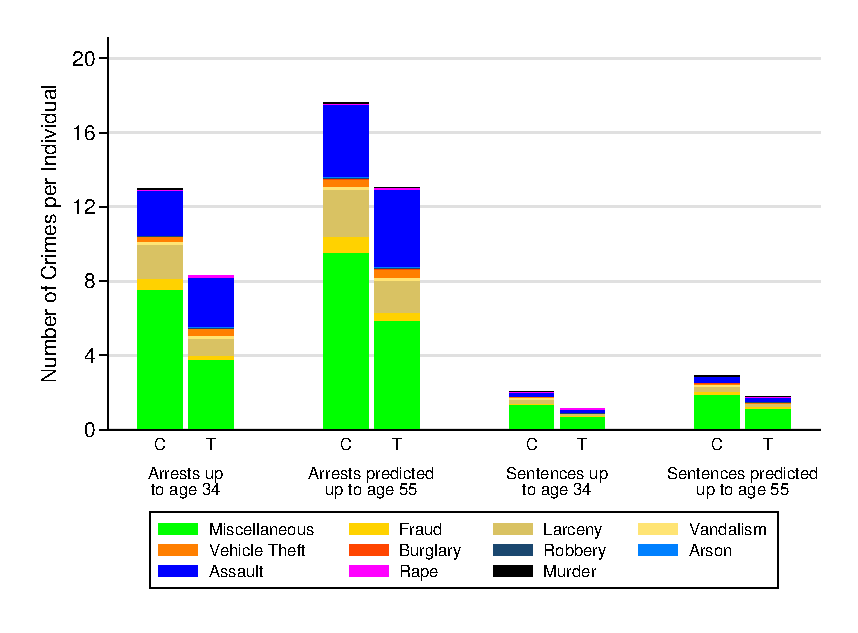
\includegraphics{AppOutput/Crime/predictions}}}
\floatfoot{
\footnotesize
\noindent Note: This figure continues Figure \ref{fig:datagraph}. It shows, for the control (C) and treatment (T) groups, the effects of adding forecasts. The first pair of columns is the same as the fifth pair of columns in Figure \ref{fig:datagraph}. The second pair of columns includes the arrests that we forecast. The third and fourth pairs of columns are the analogous pairs for sentences.
}\end{figure}

\subsection{Victimization Inflation}
\label{appendix:crime-VI}
\noindent Even though we have administrative data on crimes, we only observe the crimes that had justice system consequences (arrests or sentences). However, it is possible that the subjects committed more crimes than what we observe. Victimization Inflation (VI) is a method to capture benefits in crime reduction for crimes that did not result in justice system consequences.\footnote{\citet{Belfield_Nores_etal_2006_JHR,Heckman_Moon_etal_2010_RateofReturn}.} For most types of crimes in the U.S., there are many more victims than arrests or sentences. Using arrests as an example, VI assumes that those ``unpunished crimes'' were committed by the same people who were arrested for crimes of the same type, and in the same proportion. The calculation of VI uses as an input the national ratios of total number of reported crimes over the number of arrests. VI assumes that those national ratios are also valid for each individual. Under those assumptions, it is possible to find the total number of crimes committed by a subject for a given type of crime as the total number of arrests for that type of crime multiplied by the estimated national ratios for that type of crime. We estimate the total number of victims using two methods, one based on arrests and one based on sentences. Given that the ``unpunished'' crimes are by definition unobserved, it is not straightforward to use a data-driven method to allocate them between those subjects with arrests, those with sentences, and those with neither arrests nor sentences. We calculate separate estimates for arrests and sentences and use the average of those estimates as our main estimate. \\

\subsubsection{Construction of the Total Number of Victims in the U.S.}

\noindent The numerator of the VI ratio is an estimate of the total number of crimes of a certain crime type committed in the U.S. We construct this estimate using two datasets. First, we use the National Crime and Victimization Survey (NCVS). It has self-reported data on victimization of crimes reported on the household level. The data are available from 1995 to 2012. We also use the Uniform Crime Reporting Statistics (UCRS), which contains all crimes committed against households, individuals, and businesses that are reported to the police. These data are available from 1960 to 2013. Given that these two datasets independently underestimate the total number of crimes, but likely have significant overlap between them, we choose the highest estimate among both datasets for each type of crime. We refer to this estimate, $\overline{V_{j,t}}$, as the total number of victims in the country for type of crime $j$ in year $t$. \\

\subsubsection{Construction of the Total Number of Arrests in the U.S.}
\noindent The denominator of the VI ratio is an estimate of the total number of arrests of a certain type committed in the U.S. We have data from the ``National Arrests Analysis Tool'' of the National Bureau of Justice Statistics. These data are available from 1980 to 2012, which spans the years of all crimes that we observe in the ABC data. There is one problem with this dataset that we consider relatively minor: not all law enforcement agencies report the number of crimes (there are dozens of agencies that can legally arrest in the U.S.). However, as a large majority of them report the numbers of crimes, and because we are using national estimates, this should not greatly affect our calculations. We use these data to create $\overline{A_{j,t}}$, the total number of arrests in the country for type of crime $j$ in year $t$. \\

\subsubsection{Victimization Inflation Factors}

\noindent Figure~\ref{fig:victim1} and Figure~\ref{fig:victim2} show the VI factors calculated by year. The ratios in the charts are constructed as $r_{j,t}=\frac{\overline{V_{j,t}}}{\overline{A_{j,t}}}$. In practice, we use an average of all the yearly measures in our calculations given that this exercise imputes unobserved crimes that do not have a clearly defined date. This average of all the yearly measures is given by $r_j=\Sigma_{t=t_0}^{T}r_{j,t}/T$, and has more precise estimates of the ratio. The VI factors we use for sentences are equal to the factors used for arrests, multiplied by the arrest-sentence ratios discussed above. Below, we will discuss combining these different estimates as per our arrest-based and sentence-based methodology. For sentences, we have data from the National Judicial Reporting Program (NJRP). These data are available from 1986 onwards. Using this dataset, we construct $\overline{S_{j,t}}$, the total number of sentences in the country for type of crime $j$ in year $t$. \\

\begin{figure} [H]
\caption{Victim-arrest Ratios by Crime}
\centering \label{fig:victim1}
{\scalebox{0.8}{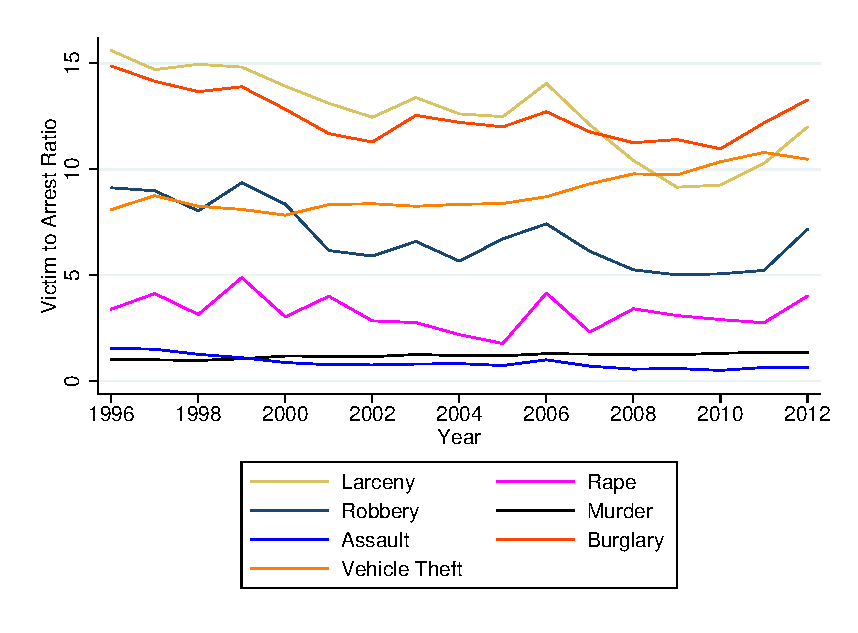
\includegraphics{AppOutput/Crime/v-to-a-ratios}}}
\floatfoot{
\footnotesize
\noindent Note: This figure shows, by year and type of crime, the number of victims (estimated from the NCVS and the UCRS datasets) divided by the number of arrests (estimated from the National Arrests Analysis Tool from the NBJS). In practice, we use a single number for each type of crime, which is an average across years.\\
}
\end{figure}

\begin{figure} [H]
\caption{Arrest-sentence Ratio by Crime}
\centering \label{fig:victim2}
{\scalebox{0.8}{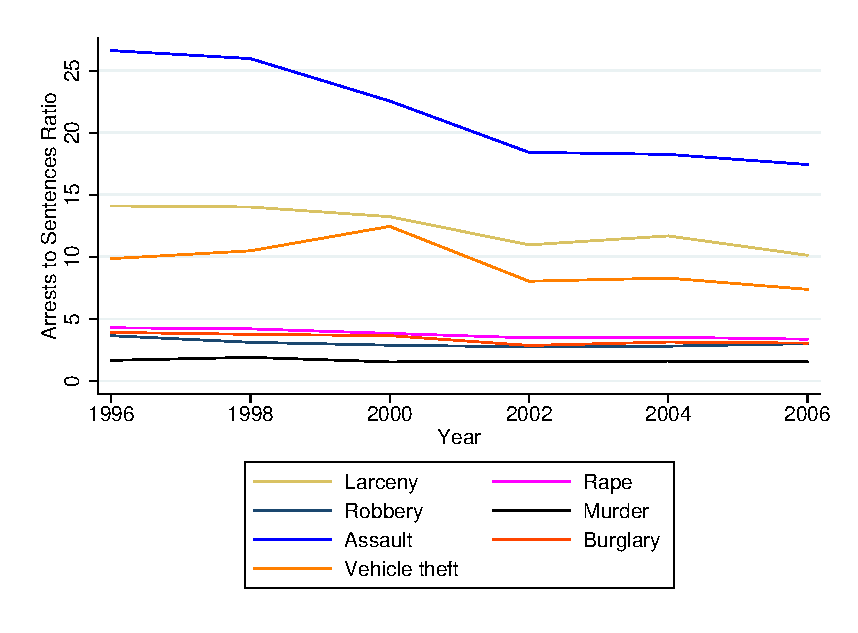
\includegraphics{AppOutput/Crime/a-to-s-ratios}}}
\floatfoot{
\footnotesize
\noindent Note: This figure shows, by year and type of crime, the number of arrests (estimated from the National Arrests Analysis Tool from the NBJS) divided by the number of sentences (estimated from the National Justice Reporting Program). In practice, we use a single number for each type of crime, which is an average across years. \\
}
\end{figure}

\subsubsection{Effects on Number of Crimes, After Victimization Inflation}
\noindent Figure \ref{fig:count-vi} shows the effects of VI on our estimates of the number of crimes committed. Note that the magnitudes in the axis are much larger than those of previous charts. The largest effects are for larceny, which is common in the data and has a victim-arrest factor of 12.6, the largest factor of all the categories of crime used in the paper. Given that the victim cost of larcenies is low, it affects the estimates less than what this chart suggests. \\

\begin{figure}[H]
\caption{Effects on Number of Crimes, After Victimization Inflation}
\centering \label{fig:count-vi}
{\scalebox{0.8}{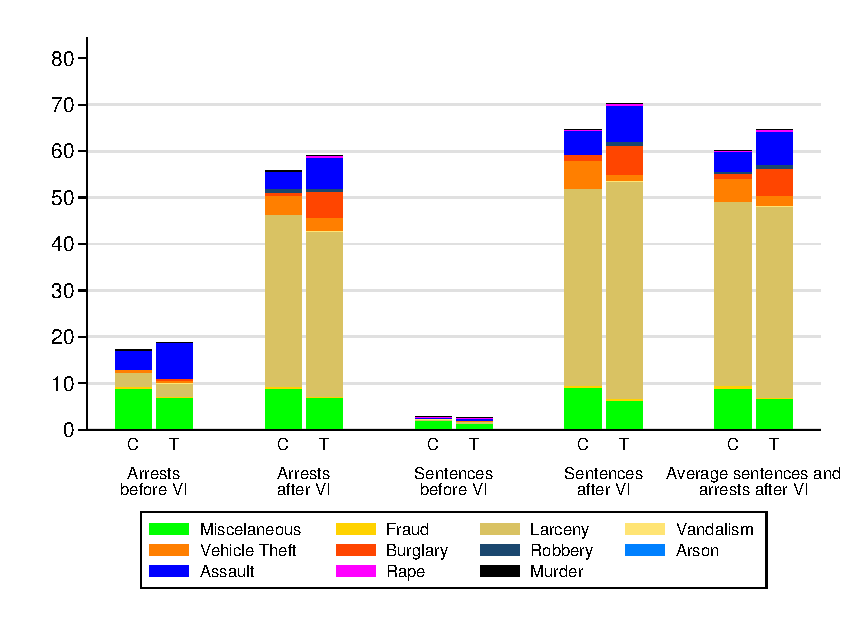
\includegraphics{AppOutput/Crime/vi}}}
\floatfoot{
\footnotesize
\noindent Note: This chart continues Figure \ref{fig:predictions}. It shows, for the control (C) and treatment (T) groups, the effects of adding victimization inflation (VI). The first pair of columns is the same as the second pair of columns in Figure \ref{fig:predictions}. The second pair of columns expand the arrests to account for VI. The third pair of columns is the same as the fourth pair of columns in Figure \ref{fig:predictions}. The fourth pair of columns expand the sentences to account for VI. The last pair of columns averages the second and the fourth pairs of columns in this chart. \\
}
\end{figure}

\noindent While the assumptions required for the victimization inflation methodology are strong, we argue that this is the best approximation for a total toll of crime's costs. The highest victim-arrest ratio shown in the figures are sensible and are not for the most costly categories of crime in the data, which stabilizes the estimates. \\

\subsection{Literature on Costs of Specific Crimes}
\noindent There are many methods to estimate unit costs of representative crimes, and many studies presenting estimates.\footnote{\citet{Cohen-Bowles_2010_Estimating-Cost-Crime} and \citet{McCollister_etal_2010_DAD} give comprehensive reviews of the state of the literature.} In this document, we only review the literature related to the inputs necessary for this paper. \\

\noindent We start by classifying the costs of crime, which is necessary to later discuss the methods to estimate the costs. Then, we present the two general types of methodologies that are used to estimate the total costs of crime: the Top-down methodologies and the Bottom-up methodologies. The former attempts to quantify the value that people put into \emph{ex-ante} prevention of crime, while the latter attempts to gather \emph{ex-post} all sources of costs that crime generates. The difference between these two methods can be large: \cite{Cohen-Bowles_2010_Estimating-Cost-Crime} show that for the particular case of estimates of the cost of rape, the top-down approach gives a value that is twice as large as the value given by most bottom-up studies. Other studies give cost estimates that are more homogeneous between these two approaches.\\

\subsubsection{Classifying the Costs of Crime}
\noindent Some methodologies used to estimate costs of crime are only able to capture some types of costs, and it might not even be clear what other methodologies are capturing. Some important types of costs are: \\
\begin{itemize}
\item Costs to the victim that can be directly quantified, such as medical bills, property losses, and lost productivity.
\item Costs to the victim that cannot be observed, such as pain and suffering.
\item Costs to the community in terms of prevention of crime, such as alarms, avoidance behavior, and police presence.
\item Costs to the community in terms of fear.
\item Costs to the community in terms of the criminal justice system, especially imprisonment.
\item Costs to the offender in terms of lowered productivity, such as forgone wages.
\end{itemize}

\subsubsection{Bottom-up (BU) Methodologies}
\noindent These approaches sum each type of cost that is imposed after the crime has been committed. The most well-known studies combine direct (also known as tangible) costs of the crimes with intangible costs. Tangible costs are everything that can be directly measured by observation, such as foregone wages, hospital costs, and police expenditure. Intangible costs are subjective, like pain and suffering. One way to measure these costs is using jury awards. For example, a jury award given as a result of an arm broken at a construction site can be used as a proxy of the intangible cost of having an arm broken in an assault.\footnote{This was first used in \citet{cohen_1988_Pain-Suffering}, and has been extensively used in BU studies after that. \citet{Miller_Cohen_ea_1996_BOOKvictim} improved on previous estimates by using jury awards specifically coming from criminal cases.} The problem of these approaches is that many of the costs of crime are not directly imposed on the victim and are hard to quantify, such as the ``fear of crime,'' the increased expenditure on crime prevention, and the negative impact of imprisonment on the community. \\

\subsubsection{Top-down (TD) Methodologies}
\noindent The other way to estimate the cost of crime is using TD methods, based on eliciting willingness to pay for avoiding crimes. The main advantage of these methods is that, in principle, they consider costs that are hard or impossible to measure directly, such as the cost of fear, avoidance behavior, and expenditures in preventative measures. There are three main methodologies for this approach, which we now briefly describe. \\

\begin{enumerate}
\item Stated Preferences. This basic method elicits the willingness to pay for hypothetical programs that would reduce crime nationwide for a sample of people.\footnote{\citet{Cohen_Rust_etal_2004_Criminology}.} Being an example of a TD methodology, it is expected that the costs obtained by this method would include factors that affect the community, and that are hard to capture, such as fear. However, it is unclear whether people consider factors like the cost of the justice system in their answers to these questions. An obvious caveat of this method is that people might not answer the real amount they would be willing to pay in these surveys.
%Then, multiplying that willingness to pay by the number individuals that would contribute, the total WTP for a certain reduction in crime is obtained. Dividing that total WTP by the number of crimes that would be avoided (number of crimes committed times the hypothetical effectiveness of the program), it is possible to find the WTP to avoid a particular crime.
\item Revealed Preferences. This method infers the value that individuals assign to crime reductions from market transactions. The most standard way to calculate these estimations is running regressions to explain the total price of houses with several factors, including the rates of crime in the area. Those parameters associated with the crime rate are considered the revealed valuation of avoiding crimes.\footnote{\citet{Thaler_1978_Value-Crime-Control}.} One weakness of this method is that it assumes that people are well-informed on the crime rates in an area. Another problem is that, in absence of extremely large and rich data on crimes and housing prices, it is not possible to separately identify the costs of different types of crimes. To the best of our knowledge, no paper has yet been able to convincingly obtain estimates per type of crime with this method.
\item Life Satisfaction. For this method, people are surveyed about their preferences between different life conditions, in which several different factors are considered. Some of those factors are income and rates of crime. By doing so, people implicitly associate monetary values to the levels of crime in the communities they would live in.\footnote{\citet{ Moore_etal_2006_Cost-of-Fear,Moore_2006_Value-Reducing-Fear}.}
\end{enumerate}

\subsubsection{Costs Used in this Study}
\noindent To summarize, both approaches have strengths and weaknesses: the TD approaches are more likely to reflect costs to the community (e.g. fear and anxiety, avoidance behavior, and protective measures) and better capture the spirit of a prevention program. However, in practice TD estimates rely on strong assumptions, and there are methodological issues associated with obtaining detailed values for the different types of crimes. It is also possible that when people answer the survey used for TD calculations they include some costs that we are including separately, such as justice system costs, and risk of death from non-murder crimes, while BU does not include them. Given those considerations, and the lack of TD costs for some categories of crime, we use BU costs for our main estimates. For completeness, we present cost estimates using both approaches. We choose \cite{Cohen_Rust_etal_2004_Criminology} as representative of the TD approaches, and \cite{McCollister_etal_2010_DAD} as representative of the BU approaches. In terms of timing, both of these studies match well with the ABC/CARE data. The bulk of crimes in the ABC/CARE data occurred between the late 1990s and early 2000s. While \cite{Cohen_Rust_etal_2004_Criminology} do not report the exact year of their survey, they use Census 2000 figures for their estimates. Even though \cite{McCollister_etal_2010_DAD} is a more recent study, many of the productivity estimates that their costs are based on are taken from papers using data from years with more crimes the late 1990s and early 2000s. The costs in those studies are presented in Table \ref{tab:individual-crime-cost}. Notice that there are some strong differences in the cost of crimes, such as assault, burglary, and especially robbery. \\

%The fact that \cite{cohen1994costs} and \cite{miller1996victim} are relatively old studies is an advantage rather than a problem. The studies better reflect the costs of crimes in those years, which are part of the period in which most crimes were committed by subjects in the ABC and CARE data. More recent estimates will be based on assumptions about productivity and costs that are not representative of the losses relevant for this study. These studies are complementary, as \cite{miller1996victim} quantifies cost to victims (productivity, medical care, mental health care, police/fire services, social services, property loss and quality of life damages), while \cite{cohen1994costs} provides a quantification of criminal justice system costs. Importantly, this study distinguishes between sources of costs, so we can impute our own cost estimates to sentences, knowing precise information about time in jail for our sample. The most recent study  \citep{mccollister2010cost} is necessary because it considers some types of crimes omitted in the previous papers.

\begin{table}[H]
\begin{threeparttable}
\caption{Unitary Costs of Crime for Victims} \label{tab:individual-crime-cost}
\begin{tabular}{lcc}
\toprule
Crime				&Top-Down Approach	&Bottom-Up Approach	\\
					& \cite{Cohen_Rust_etal_2004_Criminology}&\cite{McCollister_etal_2010_DAD}\\ \midrule
Arson				&					&12,093			\\
Assault				&95,200			&16,132 			\\
Burglary			&34,000			&1,467 			\\		
Fraud				&				&0				\\
Larceny				&				&528 				\\
Motor Vehicle Theft	&				&6,699 			\\
Murder				&13,192,000		&9,286,200 		\\
Rape				&322,320			&224,021 			\\
Robbery				&315,520			&7,273 			\\
Vandalism			&					&0				\\ \bottomrule
\end{tabular}
\begin{tablenotes}
\item Note: All amounts are in 2014 USD. The amounts reported in \cite{McCollister_etal_2010_DAD} for non-murder crimes have the extra cost for risk of death and the cost of a crime career removed (both were obtained from correspondence with the author). Risk-of-death costs do not apply, because we know the outcomes of the crimes. Crime-career costs do not apply, as we directly observe the income of the individuals. These costs also don't include police and legal system costs, as those are imputed separately and only for the cases for which individuals were arrested or sentenced.
\end{tablenotes}
\end{threeparttable}
\end{table}

\subsubsection{Timing of Effects: Incidence vs. Prevalence}
\noindent We would like to discount the costs of crime according to whether they were \textit{incurred} during a particular age of ABC/CARE subjects, because those values should be discounted at a different rate than costs incurred later, even if both costs were \textit{imposed} in the same year. Thus, the value of the imprisonment is discounted year-by-year. We have no information about the timing of costs for victims, so the value of the different crimes for the victims are discounted according to the time they were imposed (the time of the crime's occurrence). \\

\subsubsection{Costs of Imprisonment}
\noindent Unlike previous studies, we observe the sentences of the ABC/CARE subjects. This allows for a precise estimation of the costs of imprisonment. For the cost of jail and state prison, we use estimates from the \citet{US-Justice_1988_Report-Crime-Justice}. In 2014 USD, these costs are \$25,338 for a year in a state prison, and \$21,939 for a year in jail.
It is important to clarify that we only include costs of the justice system for the crimes that are known by the justice system, not for the crimes that we impute through victimization inflation. \\

%%%%%%%%%%%%%%%%%%%%%%%%%%%%%%%%%%%
\subsection{Effects on Costs of Crime}

%\subsubsection{Criminal Behavior.} The results show that there are clear reductions in the amount of crime committed between the control and treatment groups. This holds true for the majority of the categories of crime. The exceptions were Vehicle Theft, Assault, Robbery, and Arson. The visualization of the ABC and CARE data in Figure \ref{tab:lifehistory} represents the life history of each of the individuals within the ABC study that committed at least one crime, with each dot as an offense and each line as a period of incarceration. Also shown are the most serious crimes committed in the ABC data, including a habitual felon, manslaughter, and indecent liberties with children. The largest treatment effects occurred in cases of Miscellaneous, Fraud, and Larceny crimes. In sentences alone, there was a 46.3\% reduction in the number of cases, and in arrests, there was a 39\% reduction in cases for those in the treatment group compared to the control group. There are substantially fewer arrests for the individuals in the treatment group, and although there are still a few who committed a series of crimes, many did not have arrests at all.
%numbers from combined_datasetv3

\subsubsection{Effects on Costs Before Victimization Inflation}  Figure \ref{tab:diff-costs} presents the estimated costs per type of cost before victimization inflation.
\noindent There are clear positive effects for the treatment group in terms of reductions in the costs of crime. Those reductions are almost exclusively given by the large effect of the murder case we observe in the control group (note that murder also appears in the treatment group costs because of the forecasts). Comparing the bars in this figure, the costs from the justice system and from imprisonment are low compared with the victimization costs, even without victimization inflation. While the levels of the arrest-based estimates are higher than the levels of the sentence-based estimates for both the treatment and control groups, the impacts of the program are quite similar across both methods (Figure~\ref{tab:diff-costs}). \\

\begin{figure} [H]
\caption{Costs of Crime Before Victimization Inflation}
\centering  \label{tab:diff-costs}
{\scalebox{0.8}{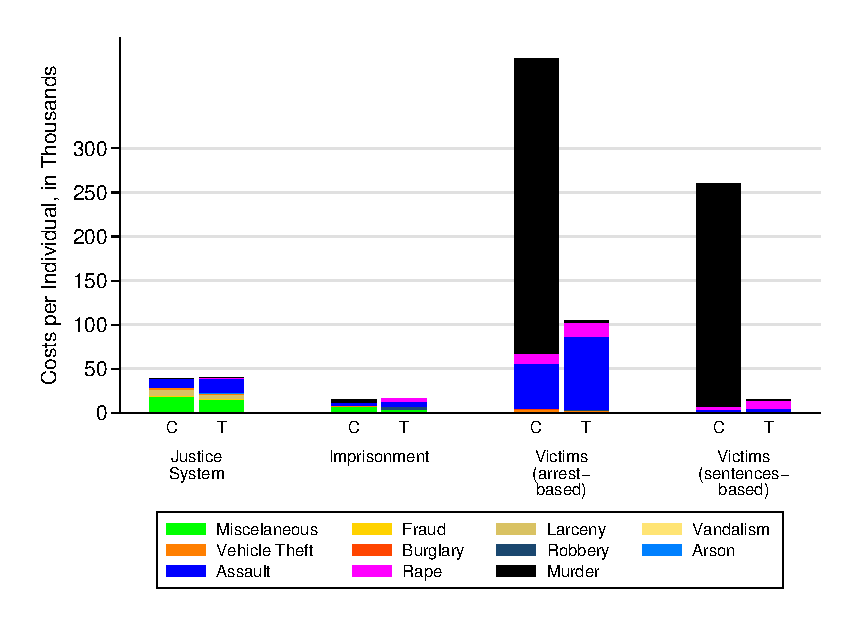
\includegraphics{AppOutput/Crime/different_costs}}}
\floatfoot{
\footnotesize
\noindent Note: This figure depicts the per capita cost for the different categories of costs and crimes we use, by control (C) and treatment (T). The first pair of columns adds up the justice system costs (including police) for all arrests inputed for each subject. The second pair of columns adds up the cost of Imprisonment. It is important to note that the costs are per capita, so there are individual cases that have much higher costs. The next two pairs of columns show the pre-victimization inflation estimates of number of crimes multiplied by the individual victim cost of the different crimes. The costs are taken from the Bottom-up approach in Table \ref{tab:individual-crime-cost}. All costs are in thousands of 2014 USD.\\
}
\end{figure}

\subsubsection{Effects on Costs After Victimization Inflation}

\noindent Figure \ref{tab:costs_vi} presents the data after applying the victimization inflation. As shown below, the inflation allows us to include a substantial amount of crime that otherwise would not have been considered. This chart shows that the treatment effects using arrest-based estimations are not substantively different from the ones using sentence-based estimations. Thus, to use all available information, we use the estimates based on the averages of the two for our analysis. \\

\begin{figure} [H]
\caption{Costs of Crime After Victimization Inflation}
\centering  \label{tab:costs_vi}
{\scalebox{0.9}{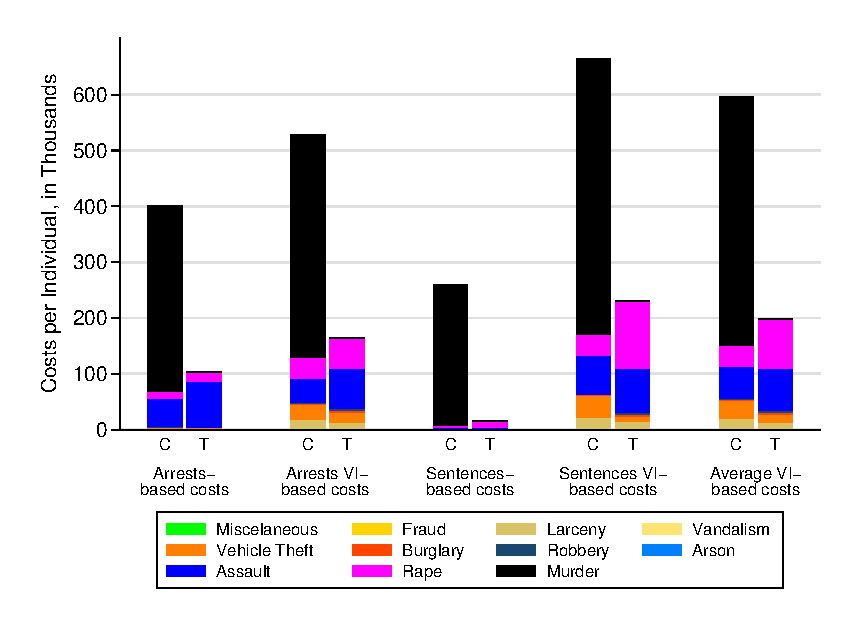
\includegraphics{AppOutput/Crime/costs_vi}}}
\floatfoot{
\footnotesize
\noindent Note: This figure depicts the per capita cost for the different categories of costs and crimes we use, by control (C) and treatment (T). The first two pairs of columns adds up all of the arrest-based costs for each subject and compares the pre- and post-victimization inflation costs. The third and fourth pair of columns compare the pre- and post-victimization inflation sentence-based costs. It is important to note that the costs are per capita, so there are individual cases that have much higher costs. The next two pairs of columns show the post-victimization inflation estimates of number of crimes multiplied by the individual victim cost of the different crimes. The costs are taken from the Bottom-up approach in Table \ref{tab:individual-crime-cost}. All costs are in thousands of 2014 USD.\\
}
\end{figure}

\noindent We consider the impact on murder as a consequence of the program rather than a statistical coincidence. We use as precedent the cost-benefit analysis of Perry in which three control group individuals and one treatment group individual committed murders.\footnote{\citet{Heckman_Moon_etal_2010_RateofReturn}.} \\

Some of the sources of cost estimates, such as the more serious crimes, result in volatile estimates due to the small sample sizes. Our estimations of the standard errors associated with the objects of interest in this paper---the present value of the program and the internal rate of return---consider those sources of volatility. Ultimately, the benefit-cost analysis is a unidimensional summary of benefits of a program, and specific flows of benefits with high variability enter naturally into the process of aggregation. \\

%\begin{table}[H]
%\begin{threeparttable}
%\caption{Effects on Total Costs}\label{tab:apx_impact-costs-total}
%{
\def\sym#1{\ifmmode^{#1}\else\(^{#1}\)\fi}
\begin{tabular}{l*{1}{ccccc}}
\hline\hline
                    &Mean Control&Mean Treatment&  Difference&           $t$& $p$-value\\
\hline
Total Costs for All Crimes&      246967&      150511&       96456&        0.64&        0.26\\
Costs Miscelaneous  &       14769&        8058&        6711&        1.45&       0.075\\
Costs Fraud         &        1095&         635&         460&        0.79&        0.21\\
Costs Larceny       &       11793&        7910&        3883&        0.83&        0.20\\
Costs Vandalism     &         260&         193&          67&        0.43&        0.34\\
Costs Vehicle Theft &       14866&       10327&        4540&        0.39&        0.35\\
Costs Burglary      &        1253&         291&         962&        1.36&       0.088\\
Costs Robbery       &        1091&        4500&       -3408&       -1.13&        0.87\\
Costs Arson         &         161&         152&          10&       0.093&        0.46\\
Costs Assault       &       38830&       33484&        5346&        0.30&        0.38\\
Costs Rape          &       35388&       65721&      -30333&       -0.43&        0.67\\
Costs Murder        &      127460&       19242&      108218&        0.87&        0.19\\
\hline\hline
\end{tabular}
}

%\begin{tablenotes}
%\item  Note: this table presents the treatment effects of ABC on total costs of crime per capita, including Victimization Inflation. All costs are in 2014 USD. We present one-sided $p$-values.
%\end{tablenotes}
%\end{threeparttable}
%\end{table}

\subsection{Sensitivity Analyses Using Alternative Cost Estimates}
\noindent So far, we study several ways to construct our estimates: \\

\begin{enumerate}
\item We show that not matching the different crime datasets could reduce the number of crimes, but that the general patterns are stable, and no dataset is especially influential.
\item We show that not including forecasts up to age 50 noticeably reduces the number of crimes, but the general patterns are not modified.
\item We show estimates using arrest-based estimations versus sentence-based estimations, and find that the differences are large in terms of the number of crimes before victimization inflation, but small after it, and do not substantially change the total benefits calculations.
\end{enumerate}

\noindent In Figure \ref{fig:costs_schedules}, we present additional deviations from our main estimates. In particular, we show how the estimations change when three different cost schedules are used: (i) Top-down costs, (ii) Bottom-up costs, and (iii) Bottom-up costs assuming that the costs of murders and rapes are identical to the cost of an assault. We also note that BU costs are a ``conservative'' option in the sense that the effects of the program are higher using TD costs. We can also see that with no murders and rapes, the effect of the program on crime is still positive, but much smaller than when those crimes are considered. \\

\begin{figure} [H]
\caption{Different Cost Schedules}
\centering  \label{fig:costs_schedules}
{\scalebox{0.9}{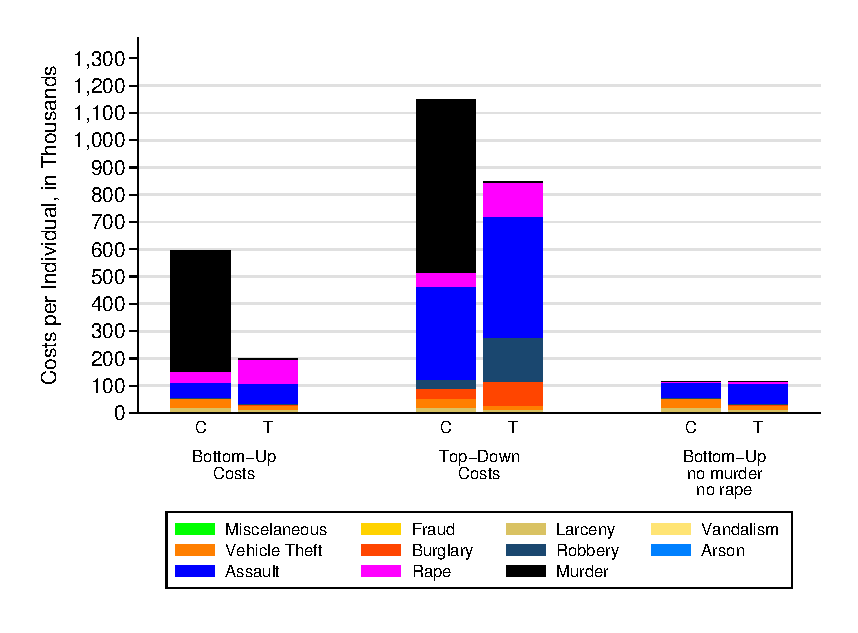
\includegraphics{AppOutput/Crime/bu_td_nomur}}}
\floatfoot{
\footnotesize
\noindent Note: This figure depicts the per capita cost for the different categories of costs and crimes we use, by control (C) and treatment (T). It presents some sensitivity analyses. The first pair of bars represents costs using the Bottom-up approach in Table \ref{tab:individual-crime-cost} to determine individual costs of crime. The second pair of bars represents costs using the Top-down approach in Table \ref{tab:individual-crime-cost} to determine individual costs of crime. The third pair of bars uses the Bottom-up approach, but replaces the values of murders and rapes with that of assaults.\\
}\end{figure}

\noindent Finally, in Figure \ref{fig:crime_discounting}, we present the effect that discounting has on our estimates that have been adjusted for deadweight loss. The first pair of bars represents the deadweight loss-adjusted cost estimates that are not discounted, and the second pair of bars represents the deadweight loss-adjusted costs that have been discounted. It is clear that the effect of discounting is substantial, approximately halving the total cost estimates.\\
% SM Comment: Discussion originally spoke about effect of adding DWL. However, this is irrelevant since both pairs have been adjusted for DWL, and thus, we cannot see impact of DWL between them.

\begin{figure} [H]
\caption{Effect of Discounting Crime Costs}
\centering  \label{fig:crime_discounting}
{\scalebox{0.9}{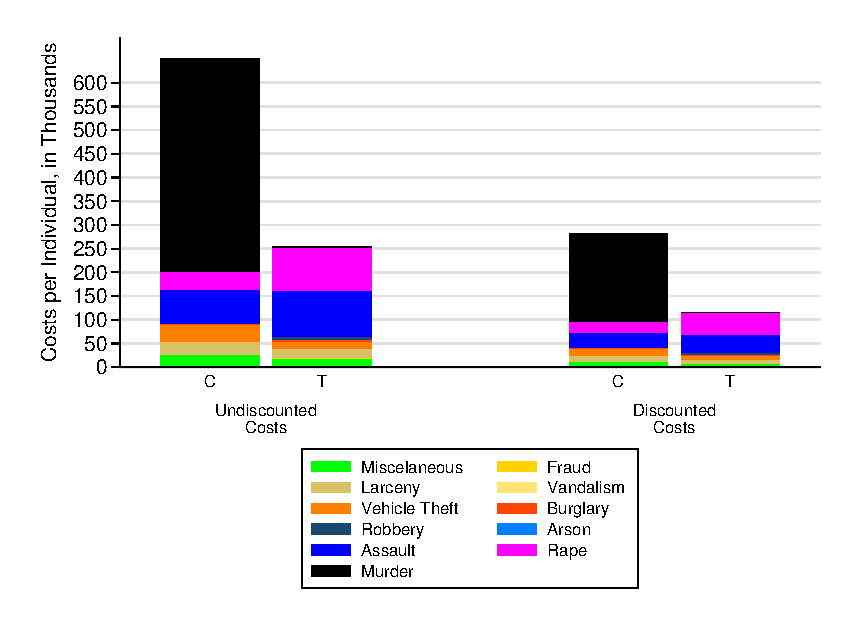
\includegraphics{AppOutput/Crime/crime_discounting}}}
\floatfoot{
\footnotesize
\noindent Note: This figure depicts the per capita cost for the different categories of costs and crimes we use, by control (C) and treatment (T). The discounted costs use 3\% as a discount factor, and are discounted to birth. The deadweight loss (DWL) adjustments increases the costs from justice system and imprisonment by 50\%. All costs are in thousands of 2014 USD.\\
}\end{figure}
